\providecommand{\toplevelprefix}{../..}  % necessary for subfile bibliography + figures compilation to work, do not move this after documentclass

\documentclass[../../book-main.tex]{subfiles}
\usepackage[UTF8]{ctex}
\graphicspath{{\subfix{../..}}}

\begin{document}

\chapter{学习线性和独立结构}
\label{ch:classic}\label{ch:linear-independent}

\begin{quote}
\hfill  ``{\em 数学艺术的本质在于发现那个蕴含了所有普遍性萌芽的特例}。''

$~$\hfill -- 大卫·希尔伯特 (David Hilbert)
\end{quote}
\vspace{5mm}

% \DP{第1节:PCA(确定性)、PPCA(统计性)、矩阵补全/RPCA(两者皆有)。添加幂迭代等。}

% \DP{第2节:正交字典学习(确定性)、伯努利-高斯ODL(统计性),允许不同类型的误差 \(\implies\) ICA(统计性)。添加幂迭代(来自\href{https://openreview.net/pdf?id=SJeY-1BKDS}{Simon的论文})。}

% \DP{第3节:使用过完备基的稀疏编码(确定性)。快速稀疏编码算法,如ISTA。如果给我基,那就是稀疏恢复问题;否则,你必须学习基(例如KSVD)。}
% \yima{实际上,John的研究小组在学习过完备字典方面有一系列工作,具有很强的正确性和理论保证。}

% \DP{写一段关于这些变体如何与核心问题相关的历史注释。}

%\DP{在第3章中,注意扩散推广了PCA(使用Peng的论文),作为在所有层面上学习去噪器。}


\textit{真实数据具有低维结构。} 要理解这一点,让我们思考一个不起眼的例子:当卫星信号不好时电视上出现的雪花。在每一帧(大约每\(\frac{1}{30}\)秒),一个尺寸为\(H \times W\)的屏幕上的RGB雪花,大致是从\([0, 1]^{3 \times H \times W}\)上的均匀分布中独立采样的。理论上,任何一帧的雪花\textit{都可能}碰巧构成一幅自然图像,但即使你花一千年时间盯着电视屏幕,这种情况也不会发生。这种差异可以用以下事实来解释:\(H \times W\)大小的自然图像集合在超立方体\([0, 1]^{3 \times H \times W}\)中只占一个极小的部分。特别是,与环境空间维度相比,它的维度极低。类似现象也发生在所有其他类型的自然数据中,如文本、音频和视频。因此,当我们设计系统和方法来处理自然数据并学习其结构或分布时,这是我们需要考虑的自然数据的一个核心属性。%\sdb{我们真的需要这个例子吗?我们已经有了\ref{sec:intro-low-dimensionality}} \DP{我觉得重申一下很好,这样可以与跳过引言的读者建立联系。另外,这个例子更贴近图像和视频,能为本书后面的部分提供动机。}

因此,我们的核心任务是学习一个在高维空间中具有低内在维度的分布。在本节的其余部分,我们将讨论几种\textit{经典}方法来完成这项任务,这些方法针对的是一些有些\textit{理想化}的数据分布模型,即几何上是线性的或统计上是独立的模型。虽然这些模型和方法本身就很重要和有用,但我们在这里讨论它们,是因为它们为更现代的、涉及深度(表示)学习的、处理更一般分布的方法提供了动机、灵感,并充当了其前身或类似物。

我们的主要方法(和一般问题表述)可以总结为:
\begin{tcolorbox}\centering
    \textbf{问题:} \textit{给定一个或多个来自数据分布的真实样本的(带噪声或不完整的)观测值,获得该样本的估计值。}
\end{tcolorbox}
这种方法是本章将要讨论的几种经典数据处理方法的基础。
\begin{itemize}
    \item 第 \ref{sec:lowrank} 节 --- 主成分分析 (PCA):给定来自一个支撑在\textit{单个低维子空间}上的分布的带噪声样本,获得位于该子空间上的真实样本的估计值。
    \item 第 \ref{sec:ica} 节 --- 完备字典学习和独立成分分析 (ICA):给定来自一个支撑在\textit{若干低维子空间的并集(\textbf{不是}张成空间)}上的分布的带噪声样本,获得真实样本的估计值。
    \item 第 \ref{sec:dictionary_learning} 节 --- 稀疏编码和过完备字典学习:给定来自一个\textit{支撑在少数非相干向量(如坐标轴)的组合}上的分布的带噪声样本,获得同样具有此性质的真实样本的估计值。
\end{itemize}
正如我们将在后续章节中揭示的,在深度学习时代,现代方法本质上采用了同样的方法进行学习。

在本章中,如上所述,我们做了一些简化的建模假设,这些假设本质上假定数据具有几何上(近似、分段)线性的结构和统计上独立的成分。在第 \ref{ch:intro} 章中,我们将这类数据模型称为“分析模型”。这些建模假设使我们能够推导出具有可证明效率保证\footnote{在数据和计算复杂度两方面。}的高效算法,以大规模处理数据。然而,对于通常复杂的现实世界数据分布来说,它们是不完美的模型,因此其基本假设只是近似成立。这意味着对这些算法的详细分析所提供的保证,在处理真实数据时也只是近似成立。尽管如此,本章讨论的技术本身就很有用,而且除此之外,它们可以说是“蕴含了普遍性萌芽的特例”,因为它们为我们稍后将要探讨的、在(深度)学习中处理更一般分布的更普适范式,提供了指导性的动机和直觉。%\sdb{感觉需要更大胆/更权威一些(更多地依赖开篇那句非常好的引言来支持)...也许可以更清楚地说明每个部分的结构?(也可以连接到第一章的“分析模型”部分)}\DP{我试了一下}


% \yima{为了与后续章节保持一致,我们可以将所有研究的模型和问题都置于同一个压缩自编码框架中:
% \begin{equation}
% \x \xrightarrow{\hspace{2mm} \mathcal{E} \hspace{2mm}}  \z \xrightarrow{\hspace{2mm} \mathcal{D} \hspace{2mm}}   \hat{\x}.    
% \end{equation}
% 我会非正式地说,本章是针对理想化的分布,这些分布允许编码器 $\mathcal{E}$ 或解码器 $\mathcal{D}$ 是\textit{浅层和线性}的。对于另一个方向,它可以通过高效的(优化)算法来实现。我甚至会进一步为每个模型和问题具体说明其相关的编码和解码算法是什么。
% }

% \yima{各位,再次强调,本章的目的不是介绍这些问题本身。我们的目标是展示如何从相同的视角和在共同的计算框架内将它们统一起来,这个框架也与未来章节的内容保持一致。}

% \sdb{我们应该根据Yi之前的评论重写这个介绍/动机部分,以帮助聚焦后面的陈述。然后相应地重写和精简PCA部分。我现在正在重写2.2节。}

%wacwwwwwwwwwwwwwwwwwwwdadw本章连接到具有低维结构的经典数据分析根源:几何线性、统计独立。



%外在/内在?表示?

%续篇中回响的三(?)件事:
%\begin{enumerate}
%    \item \textbf{我们对现实做了什么假设?} 我们的模型;数学
%        建模。
%    \item \textbf{我们如何用模型进行计算?} 简单的模型 \(\implies\)
%        高效的计算。
%    \item \textbf{它有效吗?} 当模型假设满足时 \(\implies\) 数学证明
%        它有效。(当它“还行”时 \(\implies\) 有界的“有效”)。
%\end{enumerate}
%即使模型过于理想化,其解决方案也可能传达适用于更一般情况的基本思想。

%\section{建模低维结构和分布}
%\pw{第56页、第65页缺少一些图}

\section{一个低维子空间} \label{sec:lowrank}

\subsection{主成分分析 (PCA)} \label{sub:pca}

对于低维结构,可能最简单的建模假设就是所谓的\textit{低秩}假设。设\(D\)是数据空间的维度,我们假设我们的数据属于一个维度为\(d \ll D\)的低维子空间,可能加上一些小的扰动。这个假设对于一些出人意料的复杂数据,如手写数字图像和人脸数据 \cite{BasriR2003-PAMI}(如图 \ref{fig:faces-digits} 所示),结果证明是近似成立的,而且正如我们将看到的,它非常适合进行全面的分析。

\begin{figure}
    \centering
    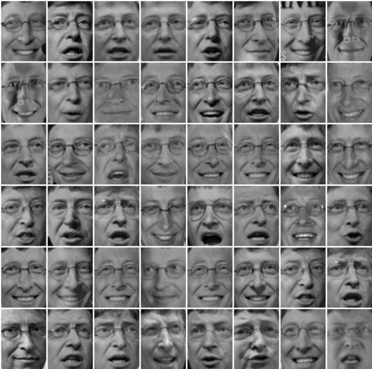
\includegraphics[width=0.4\linewidth]{\toplevelprefix/chapters/chapter2/figs/faces.png}
    \hspace{5mm} 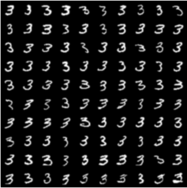
\includegraphics[width=0.395\linewidth]{\toplevelprefix/chapters/chapter2/figs/handwritten-digits.png}   
    \caption{人脸和手写数字的图像。尽管它们的外观看起来千差万别,但每一组数据都(近似地)张成一个维度非常低的(近似)线性子空间。}
    \label{fig:faces-digits}
\end{figure}

\paragraph{问题表述。}
为了用数学符号来表示,我们用一个标准正交矩阵\(\vU \in \O(D, d) \subseteq \R^{D \times d}\)来表示一个维度为\(d\)的子空间\(\cS \subseteq \R^{D}\),其中\(\vU\)的列张成\(\cS\)。然后,我们说我们的数据\(\{\vx_{i}\}_{i = 1}^{N} \subseteq \R^{D}\)具有(近似)低秩结构,如果存在一个标准正交矩阵\(\vU \in \O(D, d)\),向量\(\{\vz_{i}\}_{i = 1}^{N} \subseteq \R^{d}\),以及\textit{小的}向量\(\{\veps_{i}\}_{i = 1}^{N} \subseteq \R^{D}\),使得
\begin{equation}\label{eq:pca_dgp}
    \vx_{i} = \vU\vz_{i} + \veps_{i}, \quad \forall i \in [N].
\end{equation}
这里\(\veps_{i}\)是扰动,它使得数据不完全是低秩的;在我们的模型中包含它们,可以让我们量化在偏离模型的情况下,我们的分析在多大程度上仍然是相关的。真实的支撑子空间是\(\cS := \Range(\vU)\)。为了从这些数据中处理出所有信息,我们需要恢复\(\cS\);为此,恢复\(\vU\)就足够了,\(\vU\)也被称为\textit{主成分}。幸运的是,这是一个计算上可行的任务,名为{\bf 主成分分析},我们现在就来讨论如何解决它。

给定如\eqref{eq:pca_dgp}中分布的数据\(\{\vx_{i}\}_{i = 1}^{N}\),我们的目标是恢复模型\(\vU\)。一个自然的方法是找到子空间\(\vU^{\ast}\)和潜在向量\(\{\vz_{i}^{\ast}\}_{i = 1}^{N}\),它们能给出对\(\vx_{i} \approx \vU^{\ast}\vz_{i}^{\ast}\)的最佳近似。也就是说,我们的目标是解决以下问题:
\begin{equation}\label{eq:pca_sparse_recovery_problem}
    \min_{\tilde{\vU}, \{\tilde{\vz}_{i}\}_{i = 1}^{N}}\frac{1}{N}\sum_{i = 1}^{N}\norm{\vx_{i} - \tilde{\vU}\tilde{\vz}_{i}}_{2}^{2},
\end{equation}
其中\(\tilde{\vU}\)被约束为如上所述的标准正交矩阵。为了简洁起见,我们将在下面的类似表述中省略这个约束。

\paragraph{通过去噪进行子空间编码-解码。}
为了简化这个问题,对于一个固定的\(\tilde{\vU}\),我们有(证明作为练习):
\begin{align}
    \min_{\{\tilde{\vz}_{i}\}_{i = 1}^{N}}\frac{1}{N}\sum_{i = 1}^{N}\norm{\vx_{i} - \tilde{\vU}\tilde{\vz}_{i}}_{2}^{2} 
    &= \frac{1}{N}\sum_{i = 1}^{N}\min_{\tilde{\vz}_{i}}\norm{\vx_{i} - \tilde{\vU}\tilde{\vz}_{i}}_{2}^{2} \\
    &= \frac{1}{N}\sum_{i = 1}^{N}\norm{\vx_{i} - \tilde{\vU}\tilde{\vU}^{\top}\vx_{i}}_{2}^{2}. 
\end{align}
也就是说,上述优化问题的最优解\((\vU^{\ast}, \{\vz_{i}^{\ast}\}_{i = 1}^{N})\)满足$\vz_i^{\ast} = (\vU^{\ast})^\top\vx_i$。

现在,我们可以将原来关于\(\tilde{\vU}^{\ast}\)和\(\{\tilde{\vz}_{i}\}_{i = 1}^{N}\)的优化问题写成一个只关于\(\tilde{\vU}\)的优化问题,即,要获得基\(\vU^{\ast}\)和紧凑编码\(\{\vz_{i}^{\ast}\}_{i = 1}^{N}\),只需解决以下两个等价问题中的任意一个:
\begin{equation}\label{eq:pca_equals_denoising}
    \min_{\tilde{\vU}, \{\tilde{\vz}_{i}\}_{i = 1}^{N}}\frac{1}{N}\sum_{i = 1}^{N}\norm{\vx_{i} - \tilde{\vU}\tilde{\vz}_{i}}_{2}^{2} = \min_{\tilde{\vU}}\frac{1}{N}\sum_{i = 1}^{N}\norm{\vx_{i} - \tilde{\vU}\tilde{\vU}^{\top}\vx_{i}}_{2}^{2}.
\end{equation}
注意,\eqref{eq:pca_equals_denoising}右侧的问题是一个\textit{去噪}问题:给定低秩数据的带噪声观测\(\vx_{i}\),我们的目标是找到\(\vx_{i}\)的\textit{无噪声}副本,在模型\eqref{eq:pca_dgp}下,这个副本是$\vz_{i}$。也就是说,去噪后的输入$\hat{\vx}_i = \vU\vU^\top \vx_i$。注意到这是子空间上离$\vx_i$最近的点,如\Cref{fig:pca-geometry}所示。这里,通过解决寻找最佳子空间(由学习到的基\(\vU^{\ast}\)参数化)的等价问题,我们学习到了\textit{去噪器}的一个近似,即投影矩阵\(\vU^{\ast}(\vU^{\ast})^{\top} \approx \vU\vU^{\top}\),它将带噪声的数据点$\x_i$投影到子空间\(\cS\)上。%去噪是高维数据分析的基本构建模块之一,我们将在本书中经常讨论它,因为我们将要讨论的许多算法本质上都是针对特定数据模型(如\eqref{eq:pca_dgp},但可能更复杂一些)的去噪。

\begin{figure}
    \centering
    \begin{tikzpicture}
       \node (zero) at (0, 0) {};
       \node (u1) at (5, 1) {\(\vu_{1}\)};
       \draw[blue, ->, thick] (zero) -- (u1);
       \node[circle, inner sep=1.25pt, fill=red, draw=black] (x) at (3, 1.5) {};
       \node[circle, inner sep=1.25pt, fill=green, draw=black] (x_hat) at (3.2, 0.64)  {};
       \node at ($(x) + (0.5, 0.0)$) {\(\vx\)};
       \node at ($(x_hat) + (1, -0.2)$) {\(\hat{\vx} = \vu_{1}\vu_{1}^{\top}\vx\)};
       \draw[brown, ->, thick] (x_hat) -- (x);
       \node at (2.75, 1) {\color{brown}\(\varepsilon\)};
    \end{tikzpicture}
    \caption{\small \textbf{PCA的几何解释。} 一个数据点$\vx$(红色)被投影到由单位基向量$\vu_1$(蓝色箭头)张成的一维学习子空间上。投影$\vU\vU^\top\vx = \vu_{1}\vu_{1}^{\top}\vx$(绿色)是使用由$\vu_{1}$给出的低维结构对$\vx$进行去噪后的版本,而$\boldsymbol{\varepsilon}$(棕色箭头)表示投影残差或噪声。}
    \label{fig:pca-geometry}
\end{figure}

将上述过程整合起来,我们本质上得到了一个简单的编码-解码方案,它将一个数据点$\vx \in \R^D$映射到一个低维(潜在)空间$\R^d$,然后再映射回$\R^D$:
\begin{equation}
\x \xrightarrow{\hspace{2mm} \mathcal{E} = (\vU^\ast)^\top \hspace{2mm}}  \z \xrightarrow{\hspace{2mm} \mathcal{D} = \vU^\ast \hspace{2mm}}   \hat{\x}.  
\label{eqn:autoencoding-PCA}
\end{equation}
这里,$\vz \in \R^d$可以被看作是数据点$\x \in \R^D$的低维紧凑编码(或潜在表示),而学习到的子空间基$\vU^\ast$可以被看作是相关的码本,其列是(学习到的)最优码字。该过程通过将$\x$投影到由$\vU^\ast$张成的子空间上,实现了对$\x$的去噪功能。

\paragraph{计算子空间基。}
现在,我们继续我们的计算。设\(\vX = \mat{\vx_{1}, \dots, \vx_{N}} \in \R^{D \times N}\)是列为观测值\(\vx_{i}\)的矩阵。我们有(证明作为练习)
\begin{align}
    \argmin_{\tilde{\vU}}\frac{1}{N}\sum_{i = 1}^{N}\norm{\vx_{i} - \tilde{\vU}\tilde{\vU}^{\top}\vx_{i}}_{2}^{2}
    &= \argmax_{\tilde{\vU}}\frac{1}{N}\sum_{i = 1}^{N}\norm{\tilde{\vU}^{\top}\vx_{i}}_{F}^{2} \\ 
    &= \argmax_{\tilde{\vU}}\tr\rc{\tilde{\vU}^{\top}\bp{\frac{\vX\vX^{\top}}{N}}\tilde{\vU}}.
\end{align}
因此,为了计算主成分,我们找到使\(\tr(\tilde{\vU}^{\top}(\vX\vX^{\top}/N)\tilde{\vU})\)项最大化的正交矩阵\(\tilde{\vU}\)。我们可以通过归纳法证明,这个矩阵\(\vU^{\ast}\)的列是\(\vX\vX^{\top}/N\)的\textit{前\(d\)个单位特征向量}。我们将完整的证明留给读者在\Cref{exercise:principal-components-derivation}中完成,但我们在这里处理归纳法的基础情况。假设\(d = 1\)。那么我们只需要恢复一个单位向量\(\vu\),所以上述问题简化为
\begin{equation}
    \max_{\tilde{\vu} \colon \norm{\tilde{\vu}}_{2} = 1} \tilde{\vu}^{\top}(\vX\vX^{\top}/N)\tilde{\vu}.
\end{equation}
这就是所谓的\(\vX\vX^{\top}/N\)的\textit{瑞利商}。通过调用谱定理,我们将\(\vX\vX^{\top}/N\)对角化为\(\vV\vLambda\vV^{\top}\),其中\(\vV\)是正交的,\(\vLambda\)是对角的,其非负项。因此
\begin{equation}
    \tilde{\vu}^{\top}(\vX\vX^{\top}/N)\tilde{\vu} = \tilde{\vu}^{\top}\vV\vLambda\vV^{\top}\vu = (\vV^{\top}\tilde{\vu})^{\top}\vLambda(\vV^{\top}\tilde{\vu}).
\end{equation}
因为\(\vV\)是一个可逆的正交变换,所以\(\vV^{\top}\tilde{\vu}\)是一个单位向量,对\(\tilde{\vu}\)进行优化等价于对\(\tilde{\vw} := \vV^{\top}\tilde{\vu}\)进行优化。因此,我们可以写成
\begin{equation}
    \tilde{\vu}^{\top}(\vX\vX^{\top}/N)\tilde{\vu} = \tilde{\vw}^{\top}\vLambda\tilde{\vw},
\end{equation}
其在单位向量中的最优解\(\vw^{\star}\)是独热向量(one-hot vector),其唯一的非零(因此为单位)项位于对应于\(\vX\vX^{\top}/N\)最大特征值的索引之一。这意味着\(\tilde{\vu} = \vV\tilde{\vw}\),即原始问题的最优解,对应于\(\vX\vX^{\top}/N\)的一个单位特征向量(即\(\vV\)的一列),该特征向量对应于最大的特征值。适当地将此推广到\(d > 1\)的情况,并总结之前的所有讨论,我们得到以下非正式定理。
\begin{theorem}\label{thm:pca}
    假设我们的数据集\(\{\vx_{i}\}_{i = 1}^{N} \subseteq \R^{D}\)可以写成
    \begin{equation}
        \vx_{i} = \vU\vz_{i} + \veps_{i}, \qquad \forall i \in [N],
    \end{equation}
    其中\(\vU \in \O(D, d)\)捕捉了\textit{低秩结构},\(\{\vz_{i}\}_{i = 1}^{N} \subseteq \R^{d}\)是数据的\textit{紧凑编码},而\(\{\veps_{i}\}_{i = 1}^{N} \subseteq \R^{D}\)是表示我们的数据偏离低秩模型的小向量。那么,我们数据集的\textit{主成分}\(\vU^{\ast} \in \O(D, d)\)由\(\vX\vX^{\top}/N\)的前\(d\)个特征向量给出,其中\(\vX = [\vx_{1}, \dots, \vx_{N}] \in \R^{D \times N}\),并且近似对应于最优的线性去噪器:\(\vU^{\ast}(\vU^{\ast})^{\top} \approx \vU\vU^{\top}\)。
\end{theorem}
我们在这里不给出明确的近似率,因为它们可能变得相当技术性。在\(\veps_{i} = \vzero\)对所有\(i\)都成立的特殊情况下,学习到的\(\vU^{\ast}\)张成了样本\(\{\vx_{i}\}_{i = 1}^{N}\)的支撑集。如果此外\(\vz_{i}\)足够多样化(比如说,张成了整个\(\R^{d}\)),那么我们将实现完美恢复:\(\vU^{\ast}(\vU^{\ast}) = \vU\vU^{\ast}\)。
% \yima{上面这段的表述有些别扭……我们是把d=1情况的推导作为练习,还是在某个地方给出了推导?或者假设学生已经知道了,或者至少给了一些参考?另外,也许可以给个图来说明几何关系?}


\begin{remark}
    在一些数据分析任务中,数据矩阵\(\vX\)的格式是每个数据点作为一\textit{行}而不是像这里呈现的一\textit{列}。在这种情况下,主成分是\(\vX^{\top}\vX/N\)的前\(d\)个特征向量。
\end{remark}


\begin{remark}[通过去噪特征值进行基选择]
    在许多情况下,我们的数据要么不会真正按照子空间加噪声的模型分布,要么我们不知道子空间的真实潜在维度\(d\)。在这种情况下,我们必须选择\(d\);这个问题被称为\textit{模型选择}。在PCA的限定情况下,执行模型选择的一种方法是计算\(\vX\vX^{\top}/N\)并寻找相邻特征值急剧下降的地方;这是一个指标,表明较大特征值的索引是“真实维度\(d\)”,而\(\vX\vX^{\top}/N\)的其余特征值是由噪声或扰动\(\veps_{i}\)贡献的。模型选择是一个难题,如今在深度学习时代,它被称为“超参数优化”,通常通过暴力搜索或贝叶斯优化来完成。%\sdb{“阈值化噪声”以学习$\vU$}
\end{remark}

\begin{remark}[去噪样本]
    \eqref{eq:pca_equals_denoising}右侧的表达式,即
    \begin{equation}\label{eq:orthogonal_denoising}
        \min_{\tilde{\vU}}\frac{1}{N}\sum_{i = 1}^{N}\norm{\vx_{i} - \tilde{\vU}\tilde{\vU}^{\top}\vx_{i}}_{2}^{2},
    \end{equation}
    被称为\textit{去噪问题},之所以这么命名,是因为它是一个优化问题,其解\textit{从样本中去除噪声,使其符合子空间}。去噪——学习一个映射,从带噪声的样本中去除噪声,使其符合数据结构(如\eqref{eq:pca_dgp},但可能更复杂)——是学习分布的一种常用方法,将在续篇和整个手稿中讨论。请注意,我们已经讨论过这个概念,但由于其在后续章节中的核心重要性,值得重复。
\end{remark}

\begin{remark}[神经网络解释]
    如果我们进行PCA,我们近似恢复了由参数\(\vU_{\ast}\)编码的分布的支撑集。学习到的去噪映射则呈现为\(\vU^{\ast}(\vU^{\ast})^{\top}\)的形式。除了作为去噪器,这可以被看作是一个\textit{简单的两层权重共享线性神经网络}:第一层乘以\((\vU^{\ast})^{\top}\),第二层乘以\(\vU^{\ast}\),即
    \begin{equation}
        \operatorname{denoise}(\vx) = \underbrace{\vU^{\ast} \circ \underbrace{\id \circ \underbrace{(\vU^{\ast})^{\top}\vx}_{\text{第一“层”}}}_{\text{第一“层”的后激活}}}_{\text{“神经网络”的输出}}
    \end{equation}
    将其与一个标准的两层神经网络对比,我们看到了结构上的相似性:
\begin{equation}
\operatorname{NN}(\mathbf{x}) 
= 
\underbrace{
  \mathbf{W}^{\ast} 
  \circ 
  \bigl(
    \underbrace{
      \mathrm{ReLU} 
      \circ 
      \bigl(
        \underbrace{
          (\mathbf{U}^{\ast})^{\top} \mathbf{x}
        }_{\text{第一层}}
      \bigr)
    }_{\text{第一层的后激活}}
  \bigr)
}_{\text{神经网络的输出}}
\end{equation}

    特别是,PCA可以被解释为\textit{学习一个简单的两层去噪自编码器},\footnote{事实上,正如我们在前一章提到的,PCA是神经网络最早用来解决的问题之一 \cite{Oja1982SimplifiedNM,Baldi89}。}这是一个非平凡神经网络的最简单例子之一。在这个框架中,\textit{学习到的表示}就是\((\vU^{\ast})^{\top}\vx \approx \vz\)。通过这种方式,PCA充当了(深度)表示学习的一个模型问题,我们将在专著的后续部分进一步借鉴。请注意,在这个类比中,表示反映了输入数据,或者是输入数据朝向一个学习到的低维结构的投影。这个属性在未来将特别重要。
\end{remark}

\subsection{通过幂迭代追求低秩结构}\label{subsec:power iterations}

有一种计算效率很高的方法可以估计\(\vX\vX^{\top}/N\)或任何对称半正定矩阵\(\vM\)的最大特征向量,称为\textit{幂迭代}。这种方法是本章后面我们讨论的几种高维数据分析算法方法的基础,所以我们在这里讨论它。

现在,设\(\vM\)是一个对称半正定矩阵,存在一个由\(\vM\)的特征向量\((\vw_{i})_{i = 1}^{D}\)组成的\(\R^{D}\)的标准正交基,其对应的特征值为\(\lambda_{1} \geq \cdots \geq \lambda_{D} \geq 0\)。根据定义,任何特征向量$\vw_i$都满足$\lambda_i \vw_i = \vM \vw_i$。因此,对于任何$\lambda_i > 0$,$\vw_i$是以下方程的一个“不动点”:
\begin{equation}
    \vw = \frac{\vM\vw}{\norm{\vM\vw}_{2}}.
    \label{eqn:PCA-fixed-point}
\end{equation}

\begin{theorem}[幂迭代]
假设对于所有\(i > 1\),都有\(\lambda_{1} > \lambda_{i}\)。如果我们使用以下迭代计算\eqref{eqn:PCA-fixed-point}的不动点:
\begin{equation}\label{eq:power_iteration}
    \vv_{0} \sim \dNorm(\vzero, \vone), \qquad \vv_{t + 1} \gets \frac{\vM\vv_{t}}{\norm{\vM\vv_{t}}_{2}},
\end{equation}
那么,在极限情况下,\(\vv_{t}\)将收敛到\(\vM\)的一个最大单位范数特征向量。
\end{theorem}

\begin{proof} 首先,注意对于所有的\(t\),我们有
\begin{equation}
    \vv_{t} = \frac{\vM\vv_{t - 1}}{\norm{\vM\vv_{t - 1}}_{2}} = \frac{\vM^{2}\vv_{t - 2}}{\norm{\vM\vv_{t - 1}}_{2}\norm{\vM\vv_{t - 2}}_{2}} = \cdots = \frac{\vM^{t}\vv_{0}}{\prod_{s = 1}^{t}\norm{\vM\vv_{s}}_{2}}.
\end{equation}
因此,\(\vv_{t}\)与\(\vM^{t}\vv_{0}\)方向相同且范数为1,所以我们可以写成
\begin{equation}
    \vv_{t} = \frac{\vM^{t}\vv_{0}}{\norm{\vM^{t}\vv_{0}}_{2}}.
\end{equation}

因为$\vM$的所有特征向量\(\vw_{i}\)构成了\(\R^{D}\)的一个标准正交基,我们可以写成
\begin{equation}
    \vv_{0} = \sum_{i = 1}^{D}\alpha_{i}\vw_{i},
\end{equation}
其中因为\(\vv_{0}\)是高斯分布的,所以\(\alpha_{i}\)以概率1都是非零的。因此,我们可以用我们之前对\(\vv_{t}\)的表达式来写
\begin{equation}
    \vv_{t} = \frac{\vM^{t}\vv_{0}}{\norm{\vM^{t}\vv_{0}}_{2}} = \frac{\sum_{i = 1}^{D}\lambda_{i}^{t}\alpha_{i}\vw_{i}}{\norm{\sum_{i = 1}^{D}\lambda_{i}^{t}\alpha_{i}\vw_{i}}_{2}} = \frac{\sum_{i = 1}^{D}\lambda_{i}^{t}\alpha_{i}\vw_{i}}{\sum_{i = 1}^{D}\lambda_{i}^{t}\abs{\alpha_{i}}}. 
\end{equation}
现在,让我们考虑\(\lambda_{1} > \lambda_{2} \geq \cdots \geq \lambda_{D} \geq 0\)的情况。(具有重复最大特征值的情况类似。)那么我们可以写成
\begin{equation}
    \vv_{t} = \frac{\alpha_{1}\vw_{1} + \sum_{i = 2}^{D}(\lambda_{i}/\lambda_{1})^{t}\alpha_{i}\vw_{i}}{\abs{\alpha_{1}} + \sum_{i = 2}^{D}(\lambda_{i}/\lambda_{1})^{t}\abs{\alpha_{i}}}.
\end{equation}
因为对于所有\(i > 1\),都有\(\lambda_{1} > \lambda_{i}\),所以求和项内的项以指数速度趋于\(0\),剩下的就是极限
\begin{equation}
    \lim_{t \to \infty}\vv_{t} = \frac{\alpha_{1}}{\abs{\alpha_{1}}}\vw_{1} = \sign(\alpha_{1})\vw_{1},
\end{equation}
这是\(\vM\)的一个最大单位特征向量。 \(\vM\)的最大特征值\(\lambda_{1}\)可以通过\(\vv_{t}^{\top}\vM\vv_{t}\)来估计,它同样迅速地收敛到\(\lambda_{1}\)。
\end{proof}

% \yima{幂迭代过程与第三章中单个高斯分布的去噪过程有何关联?} \DP{关联不大,我们在第三章中讨论了这一点}

为了找到第二大特征向量,我们将幂迭代算法应用于\(\vM - \lambda_{1}\vv_{1}\vv_{1}^{\top}\),它的特征向量是\((\vw_{i})_{i = 2}^{D}\),对应的特征值是\((\lambda_{i})_{i = 2}^{D}\)。通过依次重复这个过程\(d\)次,我们可以非常高效地快速估计出\(\vM\)的前\(d\)个特征向量,对于任何对称半正定矩阵\(\vM\)都是如此。因此,我们也可以将其应用于\(\vX\vX^{\top}/N\)来恢复前\(d\)个主成分,这正是我们最初的目标。注意,这种方法一次恢复一个主成分;我们将在未来的章节中将其与其他算法方法(如对全局目标函数进行梯度下降)进行对比。

% \DP{备注:获取成分的局部迭代方法 vs 下一节(及以后)优化全局模型:这既有历史根源,也有算法上的洞见……}

% 我们在第 \ref{sec:power_iteration} 节讨论它。\sdb{我们真的想把计算推到最后吗?(我同意这是一个很好的收尾笔记;我想知道我们是否可以为每个例子讨论计算,然后在最后提供统一的解释/理解?(这可以作为本章的前瞻性结论))}



\subsection{概率PCA}\label{subsec:probabilistic PCA}

请注意,上述表述没有对数据生成过程做任何统计假设。然而,在给定的数据模型中包含统计元素是很常见的,因为它可能为分析结果增加更多有启发性的解释。因此,我们提出一个自然的问题:\textit{低维结构的统计类似物是什么?} 我们的答案是,一个低维\textit{分布}是其支撑集集中在一个低维几何结构周围的分布。

为了说明这一点,我们讨论\textit{概率主成分分析(PPCA)}。这种表述可以看作是常规PCA的一个统计变体。在数学上,我们现在将我们的数据看作是从一个取值于\(\R^{D}\)的随机变量\(\vx\)(有时也称为\textit{随机向量})中抽取的样本。我们说\(\vx\)具有(近似)低秩统计结构,当且仅当存在一个标准正交矩阵\(\vU \in \O(D, d)\),一个取值于\(\R^{d}\)的随机变量\(\vz\),以及一个取值于\(\R^{D}\)的\textit{小}随机变量\(\veps\),使得\(\vz\)和\(\veps\)是独立的,并且
\begin{equation}
    \vx = \vU\vz + \veps.
\end{equation}
我们的目标同样是恢复\(\vU\)。为此,我们设置了与子节\eqref{sub:pca}中类似的问题,即,通过对子空间支撑\(\tilde{\vU}\)和随机变量\(\vz\)进行优化来解决以下问题:
\begin{equation}
    \min_{\tilde{\vU}, \tilde{\vz}}\Ex\norm{\vx - \tilde{\vU}\tilde{\vz}}_{2}^{2}.
\end{equation}
由于我们正在寻找最好的随机变量\(\vz\),我们可以对\(\vx\)的每个值分别找到其实现\(\vz(\vx)\)。执行与子节\eqref{sub:pca}中相同的计算,我们得到 %\sdb{这里的符号很奇怪(期望里面有一个$\vz(\vx)$?并且$\vz$被重用了?)}
\begin{equation}\label{eq:ppca_denoising}
    \min_{\tilde{\vU}, \tilde{\vz}}\Ex\norm{\vx - \tilde{\vU}\tilde{\vz}}_{2}^{2} = \min_{\tilde{\vU}}\Ex\min_{\tilde{\vz}(\vx)}\norm{\vx - \tilde{\vU}\tilde{\vz}(\vx)}_{2}^{2} = \min_{\tilde{\vU}}\Ex\norm{\vx - \tilde{\vU}\tilde{\vU}^{\top}\vx}_{2}^{2},
\end{equation}
再次强调了这样一个事实:具有主成分\(\vU^{\star}\)的估计子空间对应于一个去噪器\(\vU^{\star}(\vU^{\star})^{\top}\),该去噪器投影到该子空间上。和之前一样,我们得到
\begin{align}\label{eq:PPCA}
    \argmin_{\tilde{\vU}}\Ex\norm{\vx - \tilde{\vU}\tilde{\vU}^{\top}\vx}_{2}^{2} 
    &= \argmax_{\tilde{\vU}}\Ex\norm{\tilde{\vU}^{\top}\vx}_{2}^{2} \\
    &= \argmax_{\tilde{\vU}}\tr(\tilde{\vU}^{\top}\Ex[\vx\vx^{\top}]\tilde{\vU}),
\end{align}
而后者问题的解就是二阶矩矩阵\(\Ex[\vx\vx^{\top}]\)的前\(d\)个主成分。实际上,上述问题在视觉上与前一小节中计算主成分的方程非常相似,只是用\(\Ex[\vx\vx^{\top}]\)替换了\(\vX\vX^{\top}/N\)。事实上,后一个量是前一个量的估计。两种表述实际上做的是同样的事情,并且有相同的实际解决方案——计算数据矩阵\(\vX\)的左奇异向量,或者等价地,计算估计协方差矩阵\(\vX\vX^{\top}/N\)的前几个特征向量。然而,统计表述还有一个额外的解释。假设\(\Ex[\vz] = \vzero\)和\(\Ex[\veps] = \vzero\)。我们有
\begin{equation}
    \Ex[\vx] = \vU\Ex[\vz] + \Ex[\veps] = \vzero,
\end{equation}
所以\(\Cov[\vx] = \Ex[\vx\vx^{\top}]\)。现在计算\(\Cov[\vx]\),我们有
\begin{equation}
    \Cov[\vx] = \vU\Cov[\vz]\vU^{\top} + \Cov[\veps] = \vU\Ex[\vz\vz^{\top}]\vU^{\top} + \Cov[\veps].
\end{equation}
特别地,如果\(\Cov[\veps]\)很小,那么\(\Cov[\vx] = \Ex[\vx\vx^{\top}]\)近似为一个低秩矩阵,特别是秩为\(d\)。因此\(\Ex[\vx\vx^{\top}]\)的前\(d\)个特征向量基本上概括了整个协方差矩阵。但它们也是主成分,所以我们可以将主成分分析解释为对\(\Cov[\vx]\)进行低秩分解。

\begin{remark}
    通过使用PCA的概率观点,我们对它与去噪的关系有了更清晰、更定量的理解。首先,考虑\eqref{eq:ppca_denoising}中的去噪问题,即
    \begin{equation}
        \min_{\tilde{\vU}}\Ex\norm{\vx - \tilde{\vU}\tilde{\vU}^{\top}\vx}_{2}^{2}.
    \end{equation}
    不难证明,如果\(\veps\)是一个各向同性的高斯随机变量,即其分布为\(\veps \sim \dNorm(\vzero, \sigma^{2}\vI)\),\footnote{其他分布只要支撑整个\(\R^{D}\)也行,但高斯分布在这里最容易处理。}那么对于这个问题的\textit{任何}解\(\vU^{\ast}\),我们都有
    \begin{equation}
        \vU^{\ast}(\vU^{\ast})^{\top} = \vU\vU^{\top}
    \end{equation}
    因此,真实的支撑子空间,比如\(\cS \doteq \Range(\vU)\),可以被恢复为\(\vU^{\ast}\)的列所张成的空间,因为
    \begin{equation}
        \cS = \Range(\vU) = \Range(\vU\vU^{\top}) = \Range(\vU^{\ast}(\vU^{\ast})^{\top}) = \Range(\vU^{\ast}).
    \end{equation}
    特别地,学习到的\textit{去噪映射}\(\vU^{\ast}(\vU^{\ast})^{\top}\)是到\(\cS\)上的一个正交投影,将带噪声的点推到真实的支撑子空间上。在只有有限样本的情况下,我们也可以建立一个类似的技术性结果,如\Cref{thm:pca}所示,但这需要更多的努力和技术细节。总结这一讨论,我们有以下非正式定理。
\end{remark}


\begin{theorem}\label{thm:ppca}
    假设随机变量\(\vx\)可以写成
    \begin{equation}
        \vx = \vU\vz + \veps
    \end{equation}
    其中\(\vU \in \O(D, d)\)捕捉了\textit{低秩结构},\(\vz\)是一个取值于\(\R^{d}\)的随机向量,\(\veps\)是一个取值于\(\R^{D}\)的随机向量,使得\(\vz\)和\(\veps\)独立,且\(\veps\)很小。那么,我们数据集的\textit{主成分}\(\vU^{\ast} \in \O(D, d)\)由\(\Ex[\vx\vx^{\top}]\)的前\(d\)个特征向量给出,并且近似对应于最优的线性去噪器:\(\vU^{\ast}(\vU^{\ast})^{\top} \approx \vU\vU^{\top}\)。
\end{theorem}

% \sdb{也许可以更多地讨论去噪连接的概念意义(纠正错误……链接到模型选择和基于分数的生成模型……样本复杂度和概念性见解)。也许可以针对$\vz$是高斯分布的情况来做这些?(ICA章节是“非高斯”的)}

% 本节中的其他例子也将类似。我们将介绍一个激励性的例子,以及问题的几何和统计表述。

\subsection{矩阵补全}

%\DP{待办:插入与深度学习的联系;这个过渡不是很好……}
%\yaodong{为什么把矩阵补全放在这里?}
在前面的小节中,我们讨论了\textit{学习低秩几何或统计分布}的问题,其中数据是从一个带有加性噪声的子空间中采样的。但这并不是唯一值得研究的、偏离低维分布的扰动类型。在本小节中,我们将介绍另一类在深度学习中变得越来越重要的非加性误差。让我们考虑这样一个情况:我们有一些根据\eqref{eq:pca_dgp}生成的数据\(\{\vx_{i}\}_{i = 1}^{n}\)。现在我们将它们排列成一个矩阵\(\vX = \mat{\vx_{1}, \dots, \vx_{N}} \in \R^{D \times N}\)。与之前不同,我们不能直接观测到\(\vX\);我们想象我们的观测在传输过程中被损坏了,我们得到的是
\begin{equation}
    \vY = \vM \odot \vX,
\end{equation}
其中\(\vM \in \{0, 1\}^{D \times N}\)是一个我们已知的\textit{掩码},\(\odot\)是逐元素乘法。在这种情况下,我们的目标是恢复\(\vX\)(从这一点我们可以使用PCA来恢复\(\vU_{o}\)等),而我们只拥有被损坏的观测\(\vY\)、掩码\(\vM\)以及\(\vX\)是(近似)低秩的知识。这被称为\textit{低秩矩阵补全}。

有许多优秀的资源讨论解决这个问题的算法和方法\cite{Wright-Ma-2022}。事实上,这个问题以及这个低秩结构恢复问题的类似推广,都可以通过“鲁棒PCA”来解决。我们在这里不深入探讨解决方法。相反,我们将讨论在什么条件下这个问题是\textit{有希望}解决的。一方面,在最极端的情况下,假设矩阵\(\vX\)的每个元素都是独立于其他所有元素选择的。那么即使只有一个元素缺失,我们拥有\(DN - 1\)个元素,也完全没有希望精确恢复\(\vX\)。另一方面,假设我们知道\(\vX\)的秩恰好为1,这是对数据低维结构的一个极强条件,并且我们处理的掩码是
\begin{equation}
    \vM = \mat{\vone_{(D - 1) \times 1} & \vzero_{(D - 1) \times (N - 1)} \\ 1 & \vone_{1 \times (N - 1)} }.
\end{equation}
那么我们知道数据分布在一条直线上,并且我们知道这条线上的一个向量——它就是矩阵\(\vY = \vM \odot \vX\)的第一列。从每一列的最后一个坐标(同样由掩码揭示给我们),我们可以解出每一列,因为对于每个最后的坐标,线上只有一个向量具有这个坐标。因此我们可以完美地重构\(\vX\),并且我们只需要线性的观测数量\(D + N - 1\)。

在现实世界中,实际问题介于上述两个极端情况之间。然而,这两个极端之间的差异,以及之前对PCA的讨论,揭示了一个普遍的真理核心:
\begin{quote}
    \centering
    \textit{数据分布的维度越低、结构化程度越高,处理起来就越容易,需要的观测也越少——前提是算法能有效利用这种低维结构。}
\end{quote}
正如可能预料到的,我们将在手稿的其余部分,从下一节开始,反复遇到这个主题。

% 解决这个恢复问题的一个初步想法是建立一个优化问题,其中候选解在所有未被掩码的索引处与观测值匹配,并且也具有近似低秩。这个想法可以用以下问题表述来表达:
% \begin{equation}
%     \min_{\substack{\vW \\ \vY = \vM \odot \vW}}\rank(\vW).
% \end{equation}
% 然而,这个表述遇到了两个问题:
% \begin{enumerate}
%     \item \(\rank\)函数既不连续也不凸,因此直接优化它在计算上是不可行的。
%     \item 该表述可能无法正确处理近似低秩的变量,这些变量表面上是高秩的,但实际上只是低秩加上噪声。
% \end{enumerate}
% 为了解决第一个问题,我们使用所谓的秩函数的\textit{凸松弛},即核范数\(\norm{\cdot}_{*}\),其定义为
% \begin{equation}
%     \norm{\vA}_{*} = \tr([\vA^{\top}\vA]^{1/2})
% \end{equation}
% 其中\(\vB^{1/2}\)是半正定平方根。核范数的三个关键性质是:(1) 它是一个凸函数,(2) 它构成了秩函数的一个包络,即对所有\(\vA\)都有\(\norm{\vA}_{*} \leq \rank(\vA)\),提供了一个可以有效优化的有效下界,以及(3) 它的计算也很高效。这三个性质使其成为在表述矩阵补全问题时秩函数的一个有吸引力的替代品。因此,我们使用以下问题来恢复\(\vX\):
% \begin{equation}
%     \min_{\substack{\vW \\ \vY = \vM \odot \vW}}\norm{\vW}_{*}.
% \end{equation}
% 最后,为了解决表述的第二个问题,我们使用这个问题的拉格朗日形式,得到
% \begin{equation}
%     \min_{\vW}\bc{\frac{1}{2}\norm{\vY - \vM \odot \vW}_{F}^{2} + \lambda \norm{\vW}_{*}}.
% \end{equation}
% 这个表述结果证明具有吸引人的数学性质,以及已经讨论过的概念基础。
% \sdb{这个部分感觉不太搭调……也许我们可以换个方式,通过一个关于低秩矩阵补全并非无望的基本概念性讨论,来讨论“使用低维结构纠正严重错误(缺失数据)”的想法,然后在后面谈到压缩感知时再回顾它?}

% \sdb{还要注意,一般矩阵补全之所以不平凡,是因为模型选择比小噪声PCA/去噪要困难得多……我们现在在PCA部分没有谈论模型选择。如果去掉模型选择部分,问题可能会变得足够简单,可以在这里具体地写出来。}

% \DP{如果我们知道损坏情况,我们可以使用PCA或矩阵补全;如果我们不知道,我们可以使用鲁棒PCA。一段话。}


% \begin{itemize}
%     \item 经典例子:随机噪声 \(\neq\) 相干图像 \(\implies\) 相干图像具有某种重要的结构
%     \item 如何捕捉这种结构?
%     \item 图像的正确数据结构是什么?序列呢?(如果我们能将这些动机化为子空间,那就太好了,否则就推到最后)
%     \item 朴素地:支撑在我们知道如何思考的最简单的低维对象上(子空间 \(\implies\) PCA)
%     \item 不那么朴素地:由某个易于描述的过程生成(稀疏编码、字典学习、低秩矩阵补全)
%     \item 更不朴素地:属于一个通用流形
%     \item 数据有时是从一个分布中抽取的
%     \item 最简单的低维高斯分布对应于子空间情况
%     \item 不那么简单:伯努利-高斯分布自然对应于字典学习,高斯高矩阵的外积对应于低秩矩阵
%     \item 通用的低维概率分布可以很好地被流形近似
%     \item 本节其余部分:如何在这些(最简单、不那么简单、通用)假设下进行学习——经典地
% \end{itemize}

% \DP{本小节的主要目标:连接数据的几何和统计结构;从高层次讨论数据是如何结构化的(低秩或低维流形);高斯/高斯混合假设,近似}

% \subsection{通过去噪学习线性子空间}
% 使用学习单个线性子空间的经典案例来例证通过从噪声样本中压缩(降维)来学习低维模型的通用方法。介绍幂迭代算法……

% 也许还可以连接到最近的扩散视角:当扩散-去噪过程专门用于低秩高斯的情况时,它等同于经典的PCA。还有所需样本数量的表征。

% \subsection{通过补全和纠错进行学习}
% 可能值得一提的是矩阵补全、鲁棒PCA等变体,用于在更一般的“噪声”或“扰动”概念下学习低维线性模型。

\section{完备低维子空间的混合}% 和完备字典学习 } 
\label{sec:ica}
正如我们所见,低秩信号模型足够丰富,可以全面描绘数据中的低维性与用于在误差下进行表示和恢复的高效可扩展计算算法之间的相互作用。
这些模型意味着一个\textit{线性}且对称的自编码流水线 \eqref{eqn:autoencoding-PCA}: 
\begin{equation*}
    \vz = \cE(\vx) = \vU^\top \vx, \quad \hat{\vx} = \cD(\vz) = \vU \vz,
\end{equation*}
只要$\vx$的分布确实是线性的,就可以通过主成分分析(例如,用幂方法高效求解)从$\vx$的有限样本中可证明地学习到。
这是一个限制性很强的假设——正如20世纪杰出的统计学家哈罗德·霍特林(Harold Hotelling)\footnote{巧合的是,他也因对主成分分析的发展和命名做出的贡献而闻名 \cite{Hotelling1933}。}在乔治·丹齐格(George Dantzig)首次介绍他的线性规划理论后所反对的那样 \cite{Dantzig2002-eh},
\begin{quote}
\centering
    \textit{“……我们都知道世界是非线性的。”}
\end{quote}


\begin{figure}
    \centering
    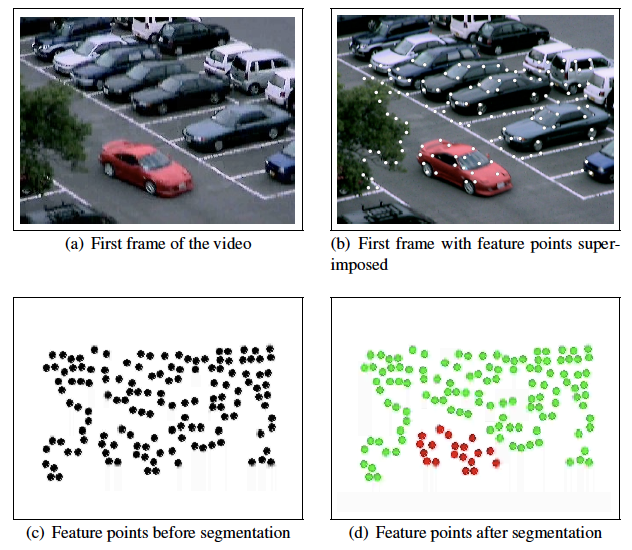
\includegraphics[height=0.35\linewidth]{\toplevelprefix/chapters/chapter2/figs/motion.png} \hspace{5mm}
    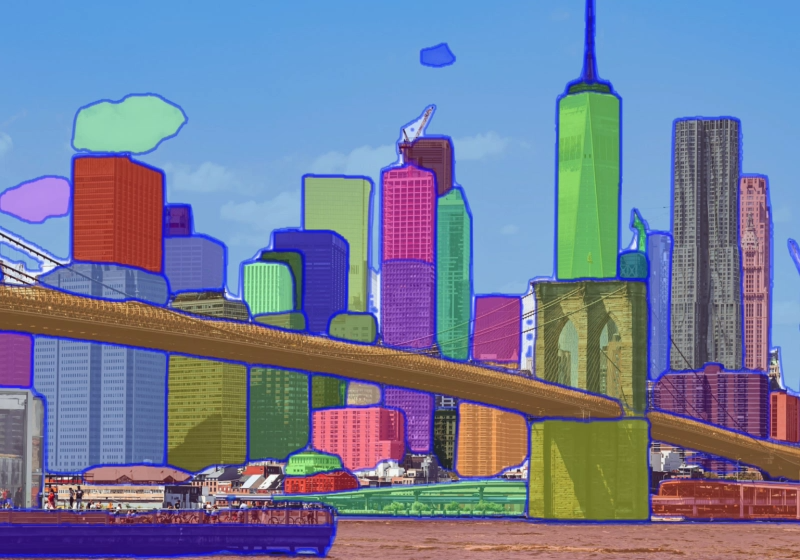
\includegraphics[height=0.349\linewidth]{\toplevelprefix/chapters/chapter2/figs/segment.png} 
    \caption{\textbf{左图:}在一个场景中独立运动的物体上跟踪的特征点。\textbf{右图:}与图像不同区域相关的图像块。}
    \label{fig:multiple-subspaces}
\end{figure}
即使考虑到其优雅和简洁性,低秩假设也过于局限,无法广泛应用于对现实世界数据的建模。
一个关键的限制是假设有一个\textit{单一}的线性子空间负责生成结构化的观测。
在许多实际应用中,由\textit{多个}不同低维子空间的\textit{混合}生成的结构提供了一个更强大、更现实的模型。
例如,考虑一个捕捉了几个不同物体运动的视频序列,每个物体都受到其独立的位移影响(图 \ref{fig:multiple-subspaces} 左)。
在对单个运动做出适当假设的情况下,每个物体在拼接的视频帧序列中都对应一个独立的低维子空间 \cite{VidalR2004-ECCV}。
再举一个例子,考虑通过学习图像中\textit{图像块}(patch,即空间上连续的像素集合)的分布模型来对自然图像进行建模(图 \ref{fig:multiple-subspaces} 右)。与我们之前看到的“特征脸”(Eigenface)例子不同,在那个例子中,姿态匹配的人脸图像可以很好地被一个单一的低维子空间近似,而自然图像中特定位置的图像块可能对应于性质非常不同的物体——例如,由于遮挡边界而导致的颜色或形状的差异。因此,用单一子空间来建模图像块的分布是徒劳的,但一个子空间的\textit{混合},每个区域一个子空间,在实践中表现出人意料地好,例如在分割或压缩方面 \cite{Mobahi-IJCV2011}。\footnote{我们将在第 \ref{ch:representation} 章回到这个观察,届时我们将展示它可以被显著推广,从而为大规模现代数据集产生强大的表示。}我们将在下一章看到一个具体的例子(例 \ref{eg:image-segmentation})。



\begin{figure}
    \centering
    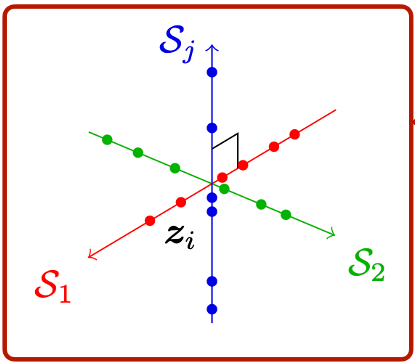
\includegraphics[height=0.35\linewidth]{\toplevelprefix/chapters/chapter2/figs/subspaces.png}
    \caption{位于低维子空间混合体上的数据,例如 $\mathcal{S}_j = \mbox{span}(\vU_j)$。}
    \label{fig:subspaces}
\end{figure}

在本节中,我们将首先讨论当数据分布具有由\textit{低维子空间混合体}建模的结构时,压缩自编码的概念和算法基础,如图 \ref{fig:subspaces} 所示。在这种情况下,解码器映射将几乎与单个子空间的情况一样简单:我们只需通过以下方式表示
\begin{equation}\label{eq:mixture-subspaces-decoder-first-cut}
    \hat{\x} = \cD(\vz) = \left( \sum_{k=1}^K \pi_k(\vz)\vU_k \right) \vz,
\end{equation}
其中 $\pi_k : \R^d \to \set{0,1}$ 是一组\textit{稀疏}的加权随机变量,使得在求和中只选择一个子空间 $\mathcal{S}_k = \mbox{span}(\vU_k)$。
然而,将这些数据 $\vx$ 编码为合适的表示 $\vz$,以及从数据中学习这样的编码器-解码器对,将被证明是更为复杂的。

我们将看到,来自\textit{稀疏表示}和\textit{独立成分分析}丰富文献的思想,如何通过稀疏性的视角,自然地重新表述上述解码器架构,以及相应的编码器架构(通过类似于主成分分析的幂方法算法获得),并为从数据中学习此类编码器-解码器对提供了强大的正确性和效率保证。从这个意义上说,混合线性低维结构的情况已经引出了我们将在本书中以更广泛的通用性发展的表示学习的许多关键要素。


%\subsection{表示子空间混合:稀疏字典}
\subsection{稀疏使用的正交字典}

%\yima{不确定为什么先介绍这个模型,而不是ICA?} \sdb{根据之前的反馈,我想把这一节从“非高斯性”(ICA的动机)转向稀疏性和几何结构。我在这节之后写ICA,但只通过BG假设,并认为这是通过稀疏性的视角来驱动的。然后算法可以像上一稿那样介绍,但没有所有抽象的峰度动机。老实说,ICA的经典动机方式对我来说似乎不太适合全局表示学习的主题(ICA的动机是:我们假设独立成分;考虑到可识别性,这意味着我们只能恢复非高斯成分;我们优化峰度来尝试找到非高斯成分)——这就是我为什么从这个模型开始。似乎子空间混合(或高斯混合)在技术上将在本书中扮演更重要的角色。}

设 $\vU_1, \dots, \vU_K$ 均为大小为 $D \times d$ 的矩阵,表示 $\R^D$ 中 $K$ 个维度为 $d$ 的子空间的一组标准正交基。
说 $\vx$ 服从由 $\vU_1, \dots, \vU_K$ 参数化的子空间混合分布,从几何上讲,意味着
\begin{equation}\label{eq:mixture-of-subspaces-geometric}
    \vx = \vU_k \vz  \quad \text{对于某个} \enspace k \in [K],\enspace \vz \in \R^d.
\end{equation}
这个几何模型的统计类似物,正如我们在PCA和线性结构案例中看到的那样,
是 $\vx$ 服从一个\textit{高斯混合}分布:也就是说,
\begin{equation}\label{eq:mixture-of-subspaces-statistical}
    \vx \sim \sum_{k=1}^K \pi_k \cN(\mathbf{0}, \vU_k\vU_k^\top), \quad \text{对于某些} \enspace \pi_k \geq 0,\enspace \sum_{k=1}^K \pi_k = 1.
\end{equation}
换句话说,对于每个 $k \in [K]$,$\vx$ 以概率 $\pi_k$ 在低维子空间 $\Span(\vU_k)$ 上服从高斯分布。
模型 \eqref{eq:mixture-of-subspaces-statistical},尽管看起来很简单,但已经足够丰富,可以作为能够扩展到大规模现代数据集的表示学习理论的基础。然而,我们必须等到第 \ref{ch:representation} 章,在我们为这个理论打下先决条件之后。

\begin{remark}[高斯混合与高斯叠加]
应该注意,上述模型 \eqref{eq:mixture-of-subspaces-statistical} 是高斯分布的混合,不要与通过叠加得到的高斯变量的混合相混淆,例如
\begin{equation}
    \vx = \sum_{i=1}^n w_i \vx_i, \quad \vx_i \sim \cN(\mathbf{0}, \vU_i\vU_i^\top),
\end{equation}
其中 $\vx_i$ 是独立的随机高斯向量,$w_i$ 是一组固定的权重。正如我们从高斯向量的性质中所知,这样的叠加 $\vx$ 仍然是一个高斯分布。
\end{remark}

目前,我们专注于 \eqref{eq:mixture-of-subspaces-geometric} 提供的几何视角。
对于这种条件表示,有一个代数上方便的替代方案。考虑一个\textit{提升的}表示向量 $\vz = [\vz_1^\top, \dots, \vz_K^\top]^\top \in \R^{dK}$,使得 $\vz$ 是\textit{$d$-稀疏}的,其支撑集位于 $dK$ 个坐标中 $K$ 个连续不重叠的 $d$ 维块之一。
那么 \eqref{eq:mixture-of-subspaces-geometric} 可以等价地写为
\begin{equation}\label{eq:mixture-of-subspaces-dictionary-pre}
    \vx = 
    \underbrace{
    \begin{bmatrix} 
    | & \hdots & |  \\
    \vU_1 & \hdots & \vU_K  \\
    | & \hdots & | 
    \end{bmatrix} 
    }_{\vU}
    \underbrace{
    \begin{bmatrix} \vz_1 \\ \vdots \\ \vz_K \end{bmatrix}
    }_{\vz},
    \quad
    \norm*{
    \begin{bmatrix} \norm*{\vz_1}_2 \\ \vdots \\ \norm*{\vz_K}_2 \end{bmatrix}
    }_0 = 1.
\end{equation}
这里,$\ell^0$“范数”$\norm{\,\cdot\,}_0$通过计算非零项的数量来衡量稀疏性:
\begin{equation}\label{eq:ell-zero-norm}
    \norm{\vz}_0 = \abs*{\set{i \given z_i \neq 0}},
\end{equation}
而矩阵 $\vU \in \R^{D \times Kd}$ 被称为一个\textit{字典},其中所有的 $\{\vU_i\}_{i=1}^K$ 都是码字。通常,如果混合中的子空间数量 $K$ 足够大,字典 $\vU$ 中包含的列数没有上限。在 $Kd < D$ 的情况下,$\vU$ 被称为\textit{欠完备}的;
当 $Kd = D$ 时,它被称为\textit{完备}的;当 $Kd > D$ 时,它被称为\textit{过完备}的。

现在,\eqref{eq:mixture-of-subspaces-dictionary-pre} 为分析的可行性提供了一个方便的松弛:与其将 $\vx$ 建模为来自 $K$ 个\textit{特定}子空间 $\vU_1, \dots, \vU_K$ 的混合,我们不如从一个字典 $\vU \in \R^{D \times m}$ 开始,其中 $m$ 可能小于或大于 $D$,并简单地寻求用足够小的稀疏度 $\norm{\vz}_0$ 来表示 $\vx = \vU \vz$。
这引出了 $\vx$ 的\textit{稀疏字典模型}:
\begin{equation}\label{eq:mixture-of-subspaces-dictionary}
    \vx =  \vU \vz + \veps,
    \quad
    \norm{\vz}_0 \ll d,
\end{equation}
其中 $\veps$ 表示一个未知的噪声向量。
从几何上看,这意味着 $\vx$ 靠近由 $\vU$ 的 $\norm{\vz}_0$ 个列组成的子集的张成空间,
这使其成为子空间混合模型 \eqref{eq:mixture-of-subspaces-geometric} 的一个实例,其中 $K$ 值非常大,并且子空间 $\vU_k$ 之间存在特定的相关性。
%尽管如此,人们发现这种松弛在简单的实际任务中很有用,并且它享有一个丰富的概念和算法理论,我们将在本章的其余部分进行发展。

%\subsection{学习稀疏使用的正交字典}

\paragraph{用于稀疏编码的正交字典。}
现在我们可以阐述我们将在本节中研究的低维子空间混合的压缩自编码问题。
我们假设我们有来自一个未知的稀疏字典模型 \eqref{eq:mixture-of-subspaces-dictionary} 的样本 $\vX = [\vx_1, \dots \vx_N]$,可能带有附加的噪声 $\veps_i$。
让我们从假设稀疏字典模型 \eqref{eq:mixture-of-subspaces-dictionary} 中的字典 $\vU$ 是完备且正交的开始,\footnote{正如我们很快将看到的,对于完备情况,做正交假设不会损失任何一般性。}并且每个系数向量 $\vz$ 是 $d$-稀疏的,其中 $d \ll D$。
此外,不失一般性地假设 $\vU$ 是一个正交矩阵(练习 \ref{exercise:whitening})。
在这种情况下,压缩自编码相当于\textit{通过优化正确地学习正交字典 $\vU$}:然后我们可以取 $\cE(\vx) = \vU^\top \vx$ 作为编码器,$\cD(\vz) = \vU \vz$ 作为解码器,并且 $\cD = \cE^{-1}$。图示如下:
% \begin{tcolorbox}
%     假设 $\vx$ 满足稀疏字典模型 \eqref{eq:mixture-of-subspaces-dictionary},其中字典 $\vU$ 是正交的,稀疏度为 $d$。
%     给定足够多的 $\vx$ 样本 $\vX = [\vx_1, \dots, \vx_N]$,
%     通过某种优化程序\textit{学习字典 $\vU$},使得
%     $\cE(\vx) = \vU^\top \vx$ 和 $\cD(\vz) = \vU \vz$ 构成 $\vx$ 上的无损自编码对。
\begin{equation}
\x \xrightarrow{\hspace{2mm} \mathcal{E} = \vU^\top \hspace{2mm}}  \z \xrightarrow{\hspace{2mm} \mathcal{D} = \vU \hspace{2mm}}   \hat{\x}.  
\label{eqn:autoencoding-DL}
\end{equation}    
% \end{tcolorbox}
我们看到,完备字典学习的自编码对 $(\cE, \cD)$ 是对称的,就像单个线性子空间的情况一样,这使得编码和解码的计算任务不比线性情况更困难。另一方面,学习字典 $\vU$ 的任务比通过PCA学习单个线性子空间要困难得多。
要理解为什么我们不能简单地使用PCA来正确学习正交字典 $\vU$,请注意,
产生PCA的损失函数,即 \eqref{eq:pca_equals_denoising},对于矩阵 $\vU$ 的行的旋转是完全不变的:也就是说,如果 $\vQ$ 是任何 $d \times d$ 的正交矩阵,那么 $\vU$ 和 $\vU \vQ$ 都是可行的,并且对于 \eqref{eq:pca_equals_denoising} 具有相同的损失。稀疏字典模型显然对这种变换不是不变的:如果我们将 $\vU$ 替换为 $\vU \vQ$ 并对表示系数 $\vz$ 进行相应的旋转 $\vQ^\top \vz$,我们就会破坏 $\vz$ 的稀疏结构,违反了建模假设。因此,我们需要开发新的算法来学习正交字典。

\subsection{完备字典学习}
\label{sec:complete-dictionary}
%\sdb{需要在这里强调低维性的作用。目前在这个模型中,低维性 \(\iff\) 稀疏性;这里只是表面上的联系}

在本节中,我们将推导解决正交字典学习问题的算法。更准确地说,我们假设观测到的向量 $\vx \in \R^D$ 遵循一个统计模型
\begin{equation}
    \vx = \vU \vz + \veps, 
    \label{eq:ica-model-ch2}
\end{equation}
其中 $\vU \in \R^{D \times D}$ 是一个未知的正交字典,$\vz$ 是一个具有统计独立分量 $z_i$ 的随机向量,每个分量均值为零,而 $\veps \in \R^D$ 是一个独立的、小的(高斯)噪声随机向量。目标是从 $\vx$ 的样本中恢复 $\vU$(并因此恢复 $\vz$)。
%模型 \eqref{eq:ica-model-ch2} 出现在诸如盲源分离等应用中,其中每个独立分量 $z_i$ 代表一个独立的源(例如音乐录音中不同乐器的声音),这些源叠加在一起产生观测值 $\vx$。
%它也是通过子空间混合模型从高维数据中提取特征的基本元操作,我们稍后会看到。

这里我们假设每个独立分量 $z_i$ 的分布为 $$z_i \sim \mathrm{Bern}(\theta) \cdot \cN(0, 1/\theta)$$。也就是说,它是一个伯努利随机变量(以概率 $\theta$ 为 $1$,以 $1-\theta$ 为 $0$)和一个独立的、方差为 $1/\theta$ 的高斯随机变量的乘积。这种分布在形式上被称为\textit{伯努利-高斯}分布。
选择这样的归一化是为了使 $\Var(z_i) = 1$,从而 $\bE[\norm{\vz}_2^2]=d$。
%利用独立性和标准高斯四阶矩为3的事实,可以计算出 $\kurt(z_i) = 3\theta(1-\theta) > 0$,所以这个模型确实适用于ICA。
这个建模假设意味着独立分量向量 $\vz$ 通常非常稀疏:
我们计算出 $\bE\left[\norm{\vz}_0\right] = d\theta$,当 $\theta$ 与 $d$ 成反比时,这个值很小。

\begin{remark}[正交假设] 
乍一看,字典 $\vU$ 是正交的这个假设似乎有些限制性。但实际上这并没有损失一般性。我们可以认为一个完备字典是任何方阵可逆矩阵 $\vU$。对于由这个字典生成的样本:$\vX = \vU \vZ \in \mathbb{R}^{D\times N}$,很容易证明\footnote{例如,参见 \cite{sun2017completeI}。},通过对数据矩阵 $\vX$ 进行一些预处理:
\begin{equation}
    \bar{\vX} = \Big(\frac{1}{N\theta} \vX\vX^\top\Big)^{-\frac{1}{2}}\vX,
\end{equation}
那么存在一个正交矩阵 $\vU_{o} \in \O(D)$ 使得
\begin{equation}
    \bar{\vX} = \vU_{o}\vZ.
\end{equation}
\end{remark}



\begin{figure}
    \centering
    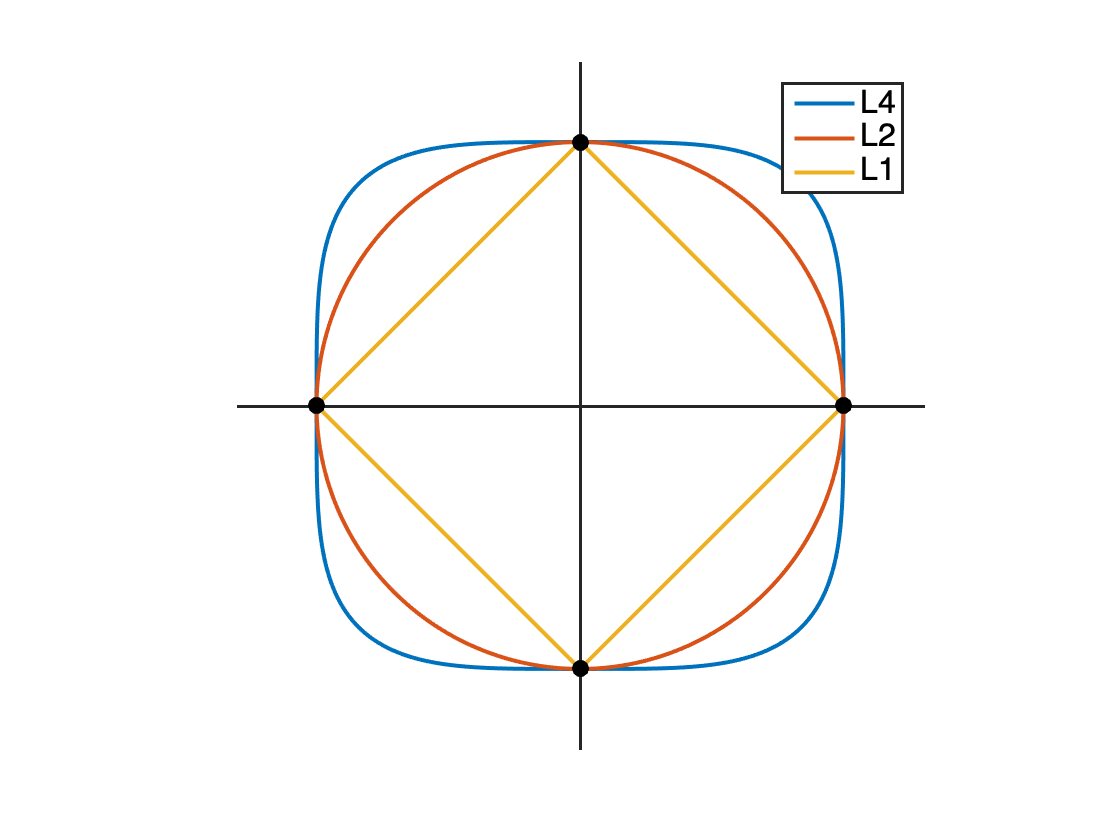
\includegraphics[width=0.6\linewidth]{\toplevelprefix/chapters/chapter2/figs/2DL4Sphere.png}\vspace{-0.1in}
    \caption{最大化 $\ell^4$ 范数或最小化 $\ell^1$ 范数都能促进稀疏性(对于球上的向量)。}
    \label{fig:L4-sphere}
\end{figure}


\paragraph{通过MSP算法进行字典学习。}

现在假设我们有一组观测数据:
\begin{equation}
    \x_i = \vU \vz_i + \veps_i,\ \forall i \in [N].
\end{equation}
设 $\vX = [\vx_1, \dots, \vx_N]$ 和 $\vZ = [\vz_1, \dots, \vz_N]$。目标是从数据 $\vX$ 中恢复 $\vU$。因此,对于任何正交矩阵 $\vA \in \O(D)$,
\begin{equation}
    \vA\vx_i = \vA\vU \vz_i + \vA\veps_i
\end{equation}
如果 $\vA = \vU^T$,那么结果将近似稀疏(因为根据假设,噪声 $\veps_i$ 的幅度很小)。

此外,鉴于 $\vU$ 是正交的且 $\veps$ 很小,向量 $\vx$ 的期望范数是可预测的,即 $\bE[\norm{\vx}_2^2] \approx \bE[\norm{\vz}_2^2]=d$。一个已知的事实是,对于球上的向量,最大化 $\ell^4$ 范数等价于最小化 $\ell^0$ 范数(以促进稀疏性),
\begin{equation}
    \argmax_{\vz \in \mathbb{S}^n}\|\vz\|_{4}\quad\Leftrightarrow\quad \argmin_{\vz \in \mathbb{S}^n}\|\vz\|_{0}.
\end{equation}
这在图 \ref{fig:L4-sphere} 中有所说明。

一个正交矩阵 $\vA$ 保持欧几里得(\(\ell^{2}\))范数:$\|\vA \x\|_2^2 = \|\x\|_2^2$。因此,为了从 $\vX$ 中找到正确的正交字典 $\vU$,我们可以尝试解决以下优化问题:
\begin{equation}\label{eq0:orthogonal-dictionary-learning-l4}
    \max_{\tilde{\vA} \in \O(D)}\,
     \frac{1}{4} \norm*{
    \tilde{\vA} \vX
    }_4^4 =  \frac{1}{4} \sum_{i=1}^N \norm*{
    \vA \vx_i
    }_4^4
\end{equation}
这被称为 $\ell^4$ 最大化问题 \cite{Zhai-2020}。在我们找到解 \(\vA^{\ast}\) 之后,我们可以取其转置 \(\vU^{\ast} = (\vA^{\ast})^{\top}\)。
\begin{remark}
    同样已知的是,对于球上的向量,最小化 $\ell^1$ 范数等价于最小化 $\ell^0$ 范数(以促进稀疏性),
\begin{equation*}
            \argmin_{\vz \in \mathbb{S}^n}\|\vz\|_{1}\quad\Leftrightarrow\quad \argmin_{\vz \in \mathbb{S}^n}\|\vz\|_{0},
\end{equation*}
这在图 \ref{fig:L4-sphere} 中也有所说明。这个事实也可以被用来有效且高效地学习字典 $\vA$。实际上,这种方法比这里使用的 $\ell^4$ 范数更早被探索。感兴趣的读者可以参考 \cite{qu2020findingsparsestvectorssubspace} 的工作。
\end{remark}

注意,上述问题等价于以下约束优化问题:
\begin{equation}\label{eq:orthogonal-dictionary-learning-l4}
    \min\,
    -   \frac{1}{4} \norm*{
    \tilde{\vA} \vX
    }_4^4 \quad \mbox{subject to} \quad  \tilde{\vA}^\top\tilde{\vA} = \vI.
\end{equation}
如 \cite{Wright-Ma-2022} 所示,使用拉格朗日乘子法,可以推导出该问题的最优解应满足以下
“不动点”条件:
\begin{equation}
    \vA^{\ast} = \mathcal{P}_{\mathrm O(D)}[( {\vA^{\ast} \vX})^{\circ3}\vX^\top],
\end{equation}
其中 $\mathcal{P}_{\mathrm O(D)}[\,\cdot\,]$ 是到正交矩阵空间 $\mathrm O(D)$ 的投影。\footnote{对于任何具有SVD分解的矩阵:$\vM = \vU\bm \Sigma \vV^\top$,$\mathcal{P}_{\mathrm O(D)}[\vM] = \vU \vV^\top$。我们将其作为练习留给读者。}

为了计算上述方程的不动点,类似于我们为PCA计算特征向量 \eqref{eqn:PCA-fixed-point} 的方式,我们可以采用以下幂迭代:
\begin{equation}\label{eq:msp_iteration}
    \vA_{t+1} = \mathcal{P}_{\mathrm O(D)}[( {\vA_t \vX})^{\circ3}\vX^\top].
\end{equation}
这被称为由 \cite{Zhai-2020} 提出的\textit{匹配、拉伸和投影}(MSP)算法。研究表明,在广泛的条件下,这种贪心算法确实以超线性速率收敛到正确的解。

\begin{remark}[$\ell^4$ 最大化的全局最优性]\label{rem:L4-global}
约束的 $\ell^4$ 最大化问题是一个非凸规划。通常不应期望任何贪心(例如梯度下降类型)算法会收敛到全局最优解。令人惊讶的是,可以证明,与一般的非凸规划不同,在球上进行 $\ell^4$ 最大化的景观
\begin{equation}\label{eq:l4-maximization-sphere}
    \min\,
    -   \frac{1}{4} \norm*{
    \vq^\top \vX
    }_4^4 \quad \mbox{subject to} \quad  \vq^\top\vq = 1.
\end{equation}
是非常良性的:所有局部最小值都接近全局最优值,并且所有临界点都是具有负曲率方向的鞍点。因此,任何具有逃离严格鞍点能力的下降方法都可以被证明找到全局最优解。有关更精确的陈述,感兴趣的读者可以参考 \cite{Qu2020Geometric}。
\end{remark}

\begin{remark}[稳定的深度线性网络]
上述计算字典的迭代过程具有一个自然的增量式“深度学习”解释。让我们定义
$\delta \vA_{t+1} = \vA_{t+1}\vA_{t}^\top$ 和 $\vZ_t = \vA_t \vX$,那么很容易证明
$$\delta \vA_{t+1} = \mathcal{P}_{\mathrm O(D)}[(\vZ_t)^{\circ3} \vZ_t^\top].$$ 
如果 $\vA_t$ 收敛到正确的字典 $\vD_o$,那么上述迭代编码过程本质上等价于一个“深度线性网络”:
$$\vZ \; \longleftarrow \; \vZ_{t+1} =  \underbrace{\delta \vA_{t+1} \delta \vA_{t} \ldots \delta \vA_{1}}_{\color{red} \text{前向构建的层}} \vX.$$
注意,每层增量变换 $\delta \vA_{t+1}$ 的计算仅依赖于前一层的特征输出 $\vZ_t$。该网络是天然稳定的,因为每一层都是一个保范数的正交变换。尽管它与线性深度网络有相似之处,但学习每一层并不需要反向传播。所有层都是在一次前向传播中学习的!
\end{remark}



% 我们现在通过一个类似于我们推导FastICA的程序,为这个目标导出一个快速的不动点算法。
% 和之前一样,我们从正交群上优化的的一阶最优性条件开始(练习 \ref{exercise:orthogonal-group-calculus}),对于峰度最大化目标,它读作
% \begin{equation}\label{eq:l4-ogrp-fxp-step1}
%     \vX \left( \vX \adj \vU \right)^{\hada 3} = \vU \underbrace{\left. \left(
%     \vU\adj \vX \left( \vX \adj \vU \right)^{\hada 3} 
%     + 
%     \left( \vU\adj \vX \right)^{\hada 3} \vX\adj \vU
%     \right) \right/ 2}_{\vS},
% \end{equation}
% 其中对称矩阵 $\vS$ 的值由约束 $\vU\adj \vU = \vI$ 决定。
% 接下来,我们回想一下,方程 \eqref{eq:l4-ogrp-fxp-step1} 被 $\ell^4$ 最大化问题的\textit{任何}临界点满足,而我们寻求一个仅由其最大化点满足的方程。
% 事实上,可以证明在 \eqref{eq:orthogonal-dictionary-learning-l4} 的任何全局最大化点 $\vU$ 处,出现在 \eqref{eq:l4-ogrp-fxp-step1} 中的矩阵 $\vS$ 实际上是半正定的,即 $\vS \succeq \mathbf{0}$(练习 \ref{exercise:l4-global-maximizers-ogrp})。使用练习 \ref{exercise:orthogonal-group-calculus} 第3部分的结果和奇异值分解,很容易
% 证明\textit{归一化} \eqref{eq:l4-ogrp-fxp-step1} 的两边会产生以下不动点表达式,在 \eqref{eq:orthogonal-dictionary-learning-l4} 的每个局部最大化点都有效:
% \begin{equation}\label{eq:l4-ogrp-fxp}
%     \mathrm{proj}_{\O(d)}\left(
%     \vX \left( \vX \adj \vU \right)^{\hada 3} 
%     \right)
%     = \vU,
% \end{equation}
% 其中我们回想一下 $\mathrm{proj}_{\O(d)}(\vX) = \vV \vW\adj$,其中 $\vX = \vV \vS \vW\adj$ 是 $\vX$ 的奇异值分解(练习 \ref{exercise:orthogonal-group-calculus} 第3部分)。
% 迭代由这个不动点表达式的左手边定义的映射,然后产生以下通过 $\ell^4$ 最大化进行完备字典学习的幂方法,称为\textit{MSP算法} \cite{Zhai2019-oc}:
% \begin{equation}
% \begin{split}\label{eq:msp}
%    \vR^+ &= \vX (\vX\adj \vU)^{\hada 3},  \\
%    \vU^+ &= \vV \vW \adj, \quad \text{其中} \enspace \vR^+ = \vV \vS \vW\adj \enspace \textit{是SVD}。
%    \end{split}
% \end{equation}
% 与之前看到的FastICA算法一样,在实践中,MSP算法极快地收敛到真实的(模对称性下的)正交字典 $\vU$。
% %即,鉴于底层目标 \eqref{eq:orthogonal-dictionary-learning-lasso} 的结构,只能恢复 $\vU$ 到其行和列的带符号排列。
% %这可以看作是我们建模假设的结果:无论是伯努利-高斯ICA建模假设还是稀疏使用字典假设(参见练习 \ref{exercise:symmetry-identifiability})。
% 在理想条件下,Zhai等人表明MSP算法 \eqref{eq:msp} 获得了三次的局部收敛速率,与FastICA算法的性能相匹配 \cite{Zhai2019-oc}。
% %同时,它在单轮优化中恢复整个字典(或在ICA背景下的混合矩阵),而所需的计算操作不比奇异值分解更昂贵,使其在实践中更可取。
% 将字典恢复问题用 $\ell^4$ 损失来表述,如在表述 \eqref{eq:orthogonal-dictionary-learning-l4} 中,还具有赋予对数据矩阵中的错误和异常值的鲁棒性的优点,正如Zhai等人所示 \cite{Zhai-2020}。

% \sdb{添加一个算法框。也许可以添加一个数值实验。}


%重要的是要认识到这个目标并不总是能够实现:例如,如果独立分量 $\vz$ 是高斯的,即 $\vz \sim \cN(\Zero, \sigma^2\vI)$,
%我们有对于任何旋转矩阵 $\vQ$(使得 $\vQ\adj \vQ = \vI$),$\vQ \vz$ 与 $\vz$ 具有相同的分布(练习),这意味着不可能从 $\vx$ 中重构 $\vz$(或者说 $\vU$)。
%这种情况被称为(统计)不可识别性;ICA仅在至多有一个高斯分量时才是可识别的。
%%即使添加了这个统计假设,请注意,也不可能从 $\vx$ 中估计独立分量的符号或能量 $\Var(z_i)$。
%%因此,为方便起见,我们将假设每个独立分量满足 $\Var(z_i)=1$,这使得独立分量在其符号上是可识别的 \cite{Hyvrinen-2000}。
%这些问题可以通过纯粹的几何概念\textit{对称性}来独立于任何对独立分量的统计模型来理解:我们在下面的练习 \ref{exercise:symmetry-identifiability} 中探讨这个问题。
%
%
%将ICA的目标与PCA的目标 \eqref{eq:pca_model} 进行对比,在PCA中,我们只是寻求用系数 $\vz$ 来\textit{表示}数据分布 $\vx$,使得
%$\vx \approx \vU \vz$。从几何上看,这对应于学习\textit{子空间} $\mathrm{col}(\vU)$,而不是特定的基 $\vU$ 本身。
%在ICA中,我们的任务正是学习特定的混合矩阵 $\vU$,或者等价地,学习独立分量 $\vz$。
%重要的是要认识到这个目标并不总是能够实现:例如,如果独立系数 $\vz$ 是高斯的,即 $\vz \sim \cN(\Zero, \sigma^2\vI)$,
%我们有对于任何旋转矩阵 $\vQ$(使得 $\vQ\adj \vQ = \vI$),$\vQ \vz$ 与 $\vz$ 具有相同的分布(练习 \ref{exercise:gaussian-rot-invar}),这意味着不可能从 $\vx$ 中重构 $\vz$(或者说 $\vU$)。
%我们称这种情况为(统计)不可识别性;ICA仅在至多有一个高斯分量时才是可识别的。
%即使添加了这个统计假设,请注意,也不可能从 $\vx$ 中估计独立分量的符号或能量 $\Var(z_i)$。
%因此,为方便起见,我们将假设每个独立分量满足 $\Var(z_i)=1$,这使得独立分量在其符号上是可识别的 \cite{Hyvrinen-2000}。
%这些问题可以通过纯粹的几何概念\textit{对称性}来独立于任何对独立分量的统计模型来理解:我们在下面的练习 \ref{exercise:symmetry-identifiability} 中探讨这个问题。
%
%给定非高斯、单位方差独立分量 $\vz$ 的高维观测 $D \geq d$,
%我们可以不失一般性地通过使用主成分分析进行降维,将我们的研究简化为 $D = d$ 的情况,正如我们在第 \ref{sub:pca} 节中所研究的。此外,通过对数据进行“白化”变换(练习 \ref{exercise:whitening}),我们可以不失一般性地假设 $\vU\adj \vU = \vI$,即 $\vU$ 是一个正交矩阵。
%



\subsection{与ICA和峰度的联系}
在伯努利-高斯模型下,变量 $z_i$ 是独立且非高斯的。那么,字典学习与经典的独立成分分析(ICA)之间存在明确的对应关系,以至于解决一个问题的算法可以用来解决另一个问题。\footnote{我们在练习 \ref{exercise:symmetry-identifiability} 中更深入地探讨了这个问题,其中建立了独立分量的非高斯性与纯粹几何概念对称性之间的联系。这个问题与我们上面观察到的PCA不适用于恢复稀疏使用的正交字典有关:在统计设置中,这可以与高斯分布的旋转不变性联系起来(练习 \ref{exercise:gaussian-rot-invar})。} 
%\sdb{添加一个BG模型/子空间图}    


为了推导一个基于ICA的算法,我们关注一个被称为\textit{峰度}的目标函数,它在ICA中被用作分量非高斯性的直接结果。一个零均值随机变量 $X$ 的\textit{峰度},或四阶累积量,定义为
\begin{equation}\label{eq:kurtosis}
\kurt(X) = \Ex{X^4} - 3 (\Ex{X^2})^2.
\end{equation}
如果我们只有来自随机变量 $X$ 的有限样本,排列成一个向量 $\vx = [x_1, \dots, x_N]$,我们通过它们的经验平均值来定义峰度,得到
\begin{equation}\label{eq:kurtosis-vector}
\kurt(\vx) = \frac{1}{N} \norm{\vx}_4^4 - \frac{3}{N^2} \norm{\vx}_2^4.
\end{equation}
最后,对于随机向量,我们将其峰度定义为每个分量标量峰度的总和。
峰度是ICA的一个自然损失函数,因为对于高斯变量 $X$,峰度为零;读者可以进一步验证伯努利-高斯分布具有正峰度。
%\sdb{我们能否通过注意到归一化使得$\ell^4$项成为相关项,从而更快地将峰度目标重塑为$\ell^4$以及与稀疏性(对偶性)的联系……?这可以变得更统一(低维性 vs 非高斯性……)}
因此,寻找非高斯独立分量的一个自然程序是搜索一组相互正交的方向 $\vV \in \R^{d \times k}$,使得 $\vV^\top \vX$ 具有最大峰度,其中 $\vX = \vU \vZ \in \R^{D \times N}$ 是伯努利-高斯ICA数据矩阵。
%通常,峰度衡量分布中异常值(或“非典型”值)的普遍性:异常值普遍性较高的分布具有正峰度,而没有的则具有负峰度。\footnote{例如,拉普拉斯分布,其与$\exp(-\norm{\vx}_1)$成正比,具有正峰度;$[-1, 1]$上的均匀分布具有负峰度。}
%\sdb{这里加个图。}
形式上,我们寻求解决以下问题
\begin{equation}
    \max_{\vV^\top \vV = \vI} \kurt(\vV^\top \vX).
\end{equation}
在一个极端情况下,我们可以设置 $k = D$ 并试图一次性恢复整个字典 $\vU$。在另一个极端情况下,我们可以设置 $k=1$ 并试图一次恢复一个方向($\vU$的一列),在找到一个方向后执行\textit{收缩}(deflation),即用 $(\vI - \vu\vu^\top) \vX$ 替换数据矩阵 $\vX$,然后再寻找另一个方向。
$k=1$ 增量方法的可扩展性与 $k=D$ 方法的效率和鲁棒性之间存在自然的权衡。因此,我们将在下面同时考虑这两种方法。

\paragraph{增量式ICA:正确性与FastICA算法。}
由Hyv\"{a}rinen和Oja \cite{hyvarinen-1997} 提出的FastICA算法,是解决ICA的 $k=1$ 峰度最大化方案的一种快速不动点算法。
当前的问题是
\begin{equation}\label{eq:kurtosis-maximization-sphere-finitesample}
    \max_{\norm{\vv}_2^2 = 1}\, \kurt(\vX^\top \vv).
\end{equation}
首先,我们将对这个目标进行一些非常基础的分析,以验证其正确性。通过变量替换 $\vw = \vU^\top \vv$,注意到这个问题等价于
\begin{equation*}
    \max_{\norm{\vw}_2^2 = 1}\, 
    \mathrm{kurt}(\vZ^\top \vw).
\end{equation*}
这个目标足够简单,以至于我们可以对其作为恢复字典 $\vU$ 的表述的正确性做出强有力的陈述。
例如,在总体设置中,即 $N \to \infty$,
我们可以使用峰度的可加性(练习 \ref{exercise:kurtosis-linearity-properties})和我们对独立分量的归一化假设,将前一个问题等价地写为
\begin{equation}\label{eq:kurtosis-maximization-sphere-population-simple}
    \max_{\norm{\vw}_2^2 = 1}\, 
    \sum_{i=1}^d \mathrm{kurt}(z_i) w_i^4.
\end{equation}
可以证明,在伯努利-高斯假设下,这个问题的优化景观是“良性的”(练习 \ref{exercise:kurtosis-sphere-landscape})——意味着目标函数的所有局部最大值都对应于恢复其中一个独立分量。
一种高效且可扩展的计算这些最大值之一的方法是通过一阶优化算法,这些算法迭代地遵循目标函数的梯度并投影到约束集 $\set{\vw \given \norm{\vw}_2^2 = 1}$ 上。
由于我们假设每个 $z_i$ 满足 $\Var(z_i)=1$,我们
对于大的 $N$ 有
\begin{equation}\label{eq:kurtosis-approximation-l4}
    \kurt(\vX^\top \vu)
    \approx
    \tfrac{1}{N} \norm{\vX^\top \vu}_4^4 - 3 \norm{\vu}_2^4.
\end{equation}
然后我们可以推导出相应的梯度近似:
\begin{equation*}
    \nabla_{\vu} \kurt(\vX^\top \vu)
    \approx
    \tfrac{4}{N} \vX (\vX^\top \vu)^{\hada 3}
    - 12 \norm{\vu}_2^2 \vu.
\end{equation*}
FastICA算法使用一种不动点方法来计算最大峰度的方向。它从峰度最大化问题的一阶最优性条件开始,给定前面的梯度近似和约束集,这些条件读作
\begin{align}\label{eq:kurtosis-max-sphere-stationarity}
   %\vP_{\vu}^\perp\left( 
   %\frac{1}{N}\vX (\vX\adj \vu)^{\hada 3} - 3 \norm{\vu}_2^2 \vu
   %\right) = \Zero
   %\iff
   \vX (\vX^\top \vu)^{\hada 3} 
   = 
   \underbrace{
   \ip*{\vu}{
   \vX (\vX^\top \vu)^{\hada 3} 
   }}_{\lambda} \vu,
   %\lambda \vu,
\end{align}
其中 $\lambda$ 的具体值由 $\vu$ 的单位范数约束确定。
练习 \ref{exercise:sphere-calculus} 描述了从第一性原理推导这些最优性条件所需的数学背景。
方程 \eqref{eq:kurtosis-max-sphere-stationarity} 被峰度最大化问题的\textit{任何}临界点满足;我们想要推导一个仅由最大化点满足的方程。
注意到 $\lambda = \norm{\vX^\top \vu}_4^4$ 后,我们等价地将 \eqref{eq:kurtosis-max-sphere-stationarity} 重新表示为修改后的方程
\begin{align}\label{eq:kurtosis-max-sphere-stationarity-modified}
   \frac{1}{N}\vX (\vX^\top \vu)^{\hada 3} 
   - 
   3 \vu
   = 
   \left(
   \frac{\lambda}{N} - 3
   \right)
   \vu,
\end{align}
并意识到 \eqref{eq:kurtosis-maximization-sphere-finitesample} 的任何最大化点
必须满足 $\lambda / N - 3 > 0$,
假设 $N$ 足够大。
因此,我们可以\textit{归一化} \eqref{eq:kurtosis-max-sphere-stationarity-modified} 的两边,
得到以下由 \eqref{eq:kurtosis-maximization-sphere-finitesample} 的每个最大化点满足的不动点方程:
\begin{align}\label{eq:kurtosis-max-sphere-fxp}
\frac{
   \frac{1}{N}\vX (\vX^\top \vu)^{\hada 3} 
   - 
   3 \vu
   }{
   \norm*{
   \frac{1}{N}\vX (\vX^\top \vu)^{\hada 3} 
   - 
   3 \vu
   }_2
   }
   =
   \vu.
\end{align}
迭代由这个不动点表达式的左手边定义的映射,然后得到Hyv\"{a}rinen和Oja的FastICA算法 \cite{hyvarinen-1997}:
\begin{equation}
\begin{split}\label{eq:fast-ica}
   \vv^+ &= \tfrac{1}{N}\vX (\vX^\top \vu)^{\hada 3}- 3 \vu
   ,  \\
   \vu^+ &= \vv^+ / \norm*{\vv^+}_2.
   \end{split}
\end{equation}
事实证明,FastICA算法收敛得非常快(实际上是\textit{三次}速率)到字典 $\vU$ 的列。
练习 \ref{exercise:fast-ica-convergence} 更深入地探讨了这些问题。\DP{引用的练习尚未完成} %\yima{缺少对练习的引用。}
将FastICA算法 \eqref{eq:fast-ica} 与在 \ref{sub:pca} 中为PCA问题研究的幂方法进行比较,我们注意到一个惊人的相似性。实际上,FastICA本质上是一个修正的幂方法,涉及经验峰度的梯度,而不是PCA目标更简单的线性梯度。

%\sdb{为FastICA添加一个算法框。}






%\subsection{通过梯度上升优化峰度来解决ICA}\label{sec:ica-via-kurtosis-gd}
%
%我们已经看到,独立分量 $\vz$ 的非高斯性是ICA问题可解的基本假设。
%我们可以进一步利用这一见解来开发计算效率高的ICA算法。
%一个零均值随机变量 $X$ 的\textit{峰度},或四阶累积量,定义为
%\begin{equation}\label{eq:kurtosis}
%\kurt(X) = \Ex{X^4} - 3 (\Ex{X^2})^2.
%\end{equation}
%如果我们只有来自随机变量 $X$ 的有限样本,排列成一个向量 $\vx = [x_1, \dots, x_N]$,我们通过它们的经验平均值来定义峰度,得到
%\begin{equation}\label{eq:kurtosis-vector}
%\kurt(\vx) = \tfrac{1}{N} \norm{\vx}_4^4 - \tfrac{3}{N^2} \norm{\vx}_2^4.
%\end{equation}
%如果 $X$ 是高斯分布,其峰度为零。通常,峰度衡量分布中异常值(或“非典型”值)的普遍性:异常值普遍性较高的分布具有正峰度,而没有的则具有负峰度。\footnote{例如,拉普拉斯分布,其与 $\exp(-\norm{\vx}_1)$ 成正比,具有正峰度;$[-1, 1]$ 上的均匀分布具有负峰度。}
%\sdb{这里加个图。}
%因此,它可以用以下程序来尝试从观测值 $\vx$ 中“挑选出”独立的非高斯分量:
%\begin{enumerate}
%    \item 使用观测数据 $\vX = [\vx_1, \dots, \vx_N]$,找到一个单位范数的方向 $\vu \in \R^d$,使得 $\vX\adj\vu$ 具有最大或最小峰度。
%    \item 执行\textit{收缩}:用找到的方向 $\vu$,从 $\vX$ 的列空间中移除 $\vu$ 以继续寻找新的方向,通过 $\vX^+ = (\vI - \vu\vu\adj) \vX$。
%    \item 重复前两个步骤,直到所有独立分量都被恢复。
%\end{enumerate}
%这种“贪心”方法,一次增量地找到一个独立分量,是ICA文献中最古老的算法之一,并且与许多其他信号处理和机器学习领域中此类贪心算法的使用相平行——从我们在第 \ref{sub:pca} 节中看到的PCA问题,到信号恢复算法如正交匹配追踪,以及优化算法如Frank-Wolfe方法 \sdb{添加引用}。
%它将ICA问题分解为多个简单的子问题,每个子问题都易于解决。
%然而,它可能导致运行时间过长,并且\textit{先验地}可能因为子问题解决不准确而导致累积错误而失败。
%我们稍后将看到如何纠正这些缺陷,至少在一般ICA问题的一个特例中。
%%\sdb{我们可以在这里做一些“历史”回顾吗——从一次一个,到“全局和切割”(一次全部,+模型选择)……}
%
%现在,让我们详细地研究上述ICA贪心程序的第一步,在“总体”情况下,即 $N \to \infty$。手头的优化问题是
%\begin{equation}\label{eq:kurtosis-maximization-sphere}
%    \max_{\norm{\vu}_2^2 = 1}\, 
%    \kurt(\ip{\vx}{\vu}).
%\end{equation}
%通过变量替换 $\vw = \vU\adj \vu$,注意到这个问题等价于
%\begin{equation*}
%    \max_{\norm{\vw}_2^2 = 1}\, 
%    \mathrm{kurt}(\ip{\vz}{\vw}).
%\end{equation*}
%使用峰度的可加性(练习 \ref{exercise:kurtosis-linearity-properties}),我们发现这个问题可以写成
%\begin{equation}\label{eq:kurtosis-maximization-sphere-population-simple}
%    \max_{\norm{\vw}_2^2 = 1}\, 
%    \sum_{i=1}^d \mathrm{kurt}(z_i) w_i^4.
%\end{equation}
%可以证明,只要至少有一个分量具有正峰度,这个问题的优化景观就是“良性的”(练习 \ref{exercise:kurtosis-sphere-landscape})——意味着目标函数的所有局部最大值都对应于恢复其中一个独立分量。
%此外,只要没有独立分量具有零峰度,像梯度下降加上少量噪声这样的自然优化算法,就能被证明在多项式时间内收敛到这些局部最大值 \cite{Jin2017-zt}。
%事实上,峰度最大化问题 \eqref{eq:kurtosis-maximization-sphere-population-simple} 甚至具有更多的结构,使得梯度下降\textit{在没有添加噪声的情况下},在对独立分量施加稍强假设的条件下,能够快速收敛到最大化点 \cite{Gilboa2019-px}。
%这些技术分析超出了我们当前讨论的范围——我们只提及它们作为一种保证,即
%我们为ICA问题开发的这些可扩展且高效的优化方法实际上是保证成功的。
%
%现在,\eqref{eq:kurtosis-maximization-sphere} 的有限样本版本是
%\begin{equation}\label{eq:kurtosis-maximization-sphere-finitesample}
%    \max_{\norm{\vu}_2^2 = 1}\, 
%    \kurt(\vX\adj \vu).
%\end{equation}
%由于我们假设每个 $z_i$ 满足 $\Var(z_i)=1$,我们
%对于大的 $N$ 有
%\begin{equation}\label{eq:kurtosis-approximation-l4}
%    \kurt(\vX\adj \vu)
%    \approx
%    \tfrac{1}{N} \norm{\vX\adj \vu}_4^4 - 3 \norm{\vu}_2^4.
%\end{equation}
%然后我们可以推导出相应的梯度近似:
%\begin{equation*}
%    \nabla_{\vu} \kurt(\vX\adj \vu)
%    \approx
%    \tfrac{4}{N} \vX (\vX\adj \vu)^{\hada 3}
%    - 12 \norm{\vu}_2^2 \vu.
%\end{equation*}
%这里,$\va^{\hada 3}$ 表示向量 $\va$ 的每个元素都取三次方。
%最后一个需要考虑的细节是解决问题 \eqref{eq:kurtosis-maximization-sphere-finitesample} 不是在环境空间 $\vu \in \R^d$ 中,而是在约束集 $\set{\vu \in \R^d \given \norm{\vu}_2^2 = 1}$ 上。
%对于 \eqref{eq:kurtosis-maximization-sphere-finitesample} 的基于梯度下降的求解器,有两个地方必须考虑到这个细节:(\sdb{如果足够相关,可以为此制作一个图……})
%\begin{enumerate}
%    \item \textbf{搜索方向:} $\R^d$ 上的梯度上升算法遵循欧几里得梯度的缩放倍数来更新当前迭代:也就是说,搜索方向是 $\eta \nabla_{\vu} \kurt(\vX\adj \vu)$,其中“步长” $\eta > 0$。
%    为了考虑约束集 $\set{\vu \in \R^d \given \norm{\vu}_2^2 = 1}$,人们不遵循梯度本身,而是其投影到一个子空间,该子空间仅表示在点 $\vu \in \set{\vu \in \R^d \given \norm{\vu}_2^2 = 1}$ 处(局部)平行于约束集的方向。
%    事实证明,对于这个球形约束集,这意味着搜索方向
%    \begin{equation}\label{eq:kurtosis-maximization-sphere-search-dir}
%        \eta \vP_{\vu}^\perp \nabla_{\vu} \kurt(\vX\adj \vu),
%    \end{equation}
%    其中 $\vP_{\vu}^\perp = \vI - \vu\vu\adj$ 是到子空间 $\Span(\set{\vu})$ 的正交补上的正交投影(练习 \ref{exercise:sphere-calculus})。
%    \item \textbf{迭代可行性:} 遵循搜索方向后,必须采取额外步骤以确保更新的迭代保持在约束集内。这可以通过投影梯度上升来实现:只需将遵循搜索方向的结果投影到约束集上。对于球形约束集,
%    这个投影由输入除以其 $\ell^2$ 范数给出:
%    \begin{equation*}
%        \mathrm{proj}_{\mathbb{S}^{d-1}}\left( \vv \right)
%        = \frac{\vv}{\norm{\vv}_2}.
%    \end{equation*}
%\end{enumerate}
%因此,我们得到以下用于解决 \eqref{eq:kurtosis-maximization-sphere-finitesample} 的梯度上升算法:
%\begin{equation}
%\begin{split}\label{eq:kurtosis-maximization-gradient-ascent}
%   \vv^+ &= \vu + \tfrac{4\eta}{N} %\left( 
%    \vP_{\vu}^\perp \vX (\vX\adj \vu)^{\hada 3}, \\
%    %- 12 \vu % \norm{\vw}_2^2 \vw
%   %\right),  \\
%   \vu^+ &= \mathrm{proj}_{\mathbb{S}^{d-1}}\left( \vv^+ \right) = \vv^+ / \norm*{\vv^+}_2.
%   \end{split}
%\end{equation}
%这里,$\eta > 0$ 是步长,如果需要,可以在迭代之间变化。
%因此,我们得到了ICA问题的第一个计算效率高的解决方案。


%\subsection{用幂方法优化峰度 (FastICA)}
%用于优化可微目标函数的基于梯度的算法,如我们用于解决ICA问题的迭代 \eqref{eq:kurtosis-maximization-gradient-ascent},在最坏情况下通常收敛速度不快于 $O(1/k)$,其中 $k$ 是迭代次数。
%在最大化点附近,这类梯度上升算法通常获得更快的\textit{线性收敛},即最坏情况下的速率为 $O(c^{k})$,其中 $0 < c < 1$ 称为(线性)收敛速率。
%然而,在像ICA这样高度结构化的信号恢复问题中,局部最优解对应于低维分布(特别是混合矩阵 $\vU$ 的特定列),
%在对数据施加温和假设的情况下,可以开发出\textit{全局}以超线性速率收敛的算法。
%我们已经在第 \ref{sub:pca} 节中看到了这样一个方法的例子,即用于主成分分析的\textit{幂方法}。
%事实上,ICA的峰度最大化问题 \eqref{eq:kurtosis-maximization-sphere-population-simple} 的并行结构也使得可以为峰度最大化推导出一个幂方法,我们现在就来讨论。
%这个推导将引导我们得到一个最初由Hyv\"{a}rinen和Oja提出的算法,称为FastICA
%\cite{hyvarinen-1997}。
%
%这个推导的关键是从不动点的角度重新考虑梯度上升更新,该更新遵循搜索
%方向 \eqref{eq:kurtosis-maximization-sphere-search-dir}。
%在这种观点下,我们将以一种形式表达问题 \eqref{eq:kurtosis-maximization-sphere-finitesample} 的一阶最优性条件,这种形式允许我们推导
%一个 \eqref{eq:kurtosis-maximization-sphere-finitesample} 的每个最大化点都必须满足的不动点方程。
%然后,我们将通过重复迭代映射的标准方法来获得解决这个不动点方程的算法。
%在当前设置中,人们从一阶平稳性条件开始
%\begin{align}\label{eq:kurtosis-max-sphere-stationarity}
%   \vP_{\vu}^\perp\left( 
%   \frac{1}{N}\vX (\vX\adj \vu)^{\hada 3} - 3 \norm{\vu}_2^2 \vu
%   \right) = \Zero
%   \iff
%   \vX (\vX\adj \vu)^{\hada 3} 
%   = 
%   \underbrace{
%   \ip*{\vu}{
%   \vX (\vX\adj \vu)^{\hada 3} 
%   }}_{\lambda} \vu,
%   %\lambda \vu,
%\end{align}
%其中 $\lambda$ 的具体值由单位范数约束确定。
%方程 \eqref{eq:kurtosis-max-sphere-stationarity} 被峰度最大化问题的\textit{任何}临界点满足;我们想要推导一个仅由最大化点满足的方程。
%注意到 $\lambda = \norm{\vX\adj \vu}_4^4$ 后,我们等价地将 \eqref{eq:kurtosis-max-sphere-stationarity} 重新表示为修改后的方程
%\begin{align}\label{eq:kurtosis-max-sphere-stationarity-modified}
%   \frac{1}{N}\vX (\vX\adj \vu)^{\hada 3} 
%   - 
%   3 \vu
%   = 
%   \left(
%   \frac{\lambda}{N} - 3
%   \right)
%   \vu,
%\end{align}
%并意识到 \eqref{eq:kurtosis-maximization-sphere-finitesample} 的任何最大化点
%必须满足 $\lambda / N - 3 > 0$
%(假设 $N$ 足够大且至少有一个 $i$ 使得 $\kurt(z_i) > 0$,从而使问题非平凡)。
%因此,我们可以\textit{归一化} \eqref{eq:kurtosis-max-sphere-stationarity-modified} 的两边,
%得到以下由 \eqref{eq:kurtosis-maximization-sphere-finitesample} 的每个最大化点满足的不动点方程:
%\begin{align}\label{eq:kurtosis-max-sphere-fxp}
%\frac{
%   \frac{1}{N}\vX (\vX\adj \vu)^{\hada 3} 
%   - 
%   3 \vu
%   }{
%   \norm*{
%   \frac{1}{N}\vX (\vX\adj \vu)^{\hada 3} 
%   - 
%   3 \vu
%   }_2
%   }
%   =
%   \vu.
%\end{align}
%迭代由这个不动点表达式的左手边定义的映射,然后得到Hyv\"{a}rinen和Oja的FastICA算法 \cite{hyvarinen-1997}:
%\begin{equation}
%\begin{split}\label{eq:fast-ica}
%   \vv^+ &= \tfrac{1}{N}\vX (\vX\adj \vu)^{\hada 3}- 3 \vu
%   ,  \\
%   \vu^+ &= \vv^+ / \norm*{\vv^+}_2.
%   \end{split}
%\end{equation}
%尽管我们的推导依赖于不动点条件 \eqref{eq:kurtosis-max-sphere-fxp} 对于点 $\vu$ 成为峰度最大化问题最大化点的\textit{必要性},而不是其充分性,但事实证明,FastICA算法确实以极快的速度(实际上是超线性的\textit{三次}速率)收敛到理想的解,即混合矩阵 $\vU$ 的列。
%唯一需要提及的警告是,它不一定收敛到问题 \eqref{eq:kurtosis-maximization-sphere-finitesample} 的解:在适当的假设下,它将收敛到与具有最大绝对峰值的独立分量 $z_i$ 相关联的 $\vU$ 的列,这在ICA的设置中是一个可接受的结果。
%练习 \ref{exercise:fast-ica-convergence} 更深入地探讨了这些问题。
%
%将FastICA算法 \eqref{eq:fast-ica} 与在 \ref{sub:pca} 中为PCA问题研究的幂方法进行比较,我们注意到一个惊人的相似性。实际上,FastICA本质上是一个修正的幂方法,涉及经验峰度的梯度,而不是PCA目标更简单的线性梯度。
%%这是单分量峰度最大化问题 \eqref{eq:kurtosis-maximization-sphere-finitesample} 的一个\textit{幂方法}的例子。
%我们很快将看到这类算法在快速收敛到低维结构方面的更多用例和适用性。

%\sdb{可以写一些关于ICA的其他方法吗?可能与最大互信息有关(可以在别处联系,例如,下一章/压缩?)}

%\subsection{完备字典学习}
%
%为了更深入地理解ICA问题的几何意义,特别是其作为单低秩子空间PCA模型的推广的作用,关注
%独立分量 $\vz$ 的一个特定统计模型是有帮助的。
%这里,我们假设每个独立分量的分布为 $\mathrm{Bern}(\theta) \cdot \cN(0, 1/\theta)$:也就是说,是一个伯努利随机变量(概率 $\theta$ 为 $1$,概率 $1-\theta$ 为 $0$)和一个独立的、方差为 $1/\theta$ 的高斯随机变量的乘积。选择这样的归一化是为了使 $\Var(z_i) = 1$,从而 $\bE[\norm{\vz}_2^2]=d$。利用独立性和标准高斯四阶矩为3的事实,可以计算出 $\kurt(z_i) = 3\theta(1-\theta) > 0$,所以这个模型确实适用于ICA。
%
%注意到这个建模假设意味着独立分量向量 $\vz$ 通常\textit{非常稀疏},即具有少量非零项(图 \ref{} \sdb{添加一个BG模型/子空间图})。
%我们通过其所谓的 $\ell^0$ 范数来衡量向量的稀疏性,该范数计算向量的非零项数量:
%很容易计算出 $\bE\left[\norm{\vz}_0\right] = d\theta$,所以当伯努利
%率参数 $\theta$ 被选择为与 $d$ 成反比时,独立分量向量 $\vz$ 确实通常非常稀疏 \sdb{为了让 $\vz$ 稀疏,你需要选择例如 $\theta = 2/d$,这意味着每个项相关的高斯分布的方差是 $d/2$(非常大),这可能感觉有点奇怪。这是因为坚持归一化使得 $\Var(z_i) = 1$。我认为这种坚持是有道理的,因为它有助于本节的推导。但值得注意和反思(告诉我你的想法)。}
%因为 $\vz$ 的每个分量都是\textit{独立的},所以观测值 $\vx$ 的实现因此对应于混合矩阵 $\vU$ 的少量列的线性组合。这意味着观测值是从一个\textit{子空间的混合}中抽取的,由(通常)$\vU$ 的至多 $\bE\left[\norm{\vz}_0\right]$ 列的所有可能选择来参数化(图 \ref{} \sdb{添加图;双面板之前……})。
%
%这种几何视角对应于一个高度相关的模型和问题族,称为\textit{字典学习}。在这里,观测值 $\vx$ 被看作是“字典”即矩阵 $\vU$ 的少量“原子”(列)的稀疏线性组合。
%目标与ICA问题 \eqref{eq:ica-model-ch2} 相同,但解决字典学习问题的算法利用了向量 $\vz$ 是稀疏的底层几何假设,而不是像ICA中那样利用其分量的独立性。
%在当前设置中,字典 $\vU$ 是一个正交矩阵(或更一般地,一个满秩方阵),具体的恢复问题被称为\textit{完备字典学习}。
%当 $d > D$ 时,称为\textit{过完备}字典学习——我们将在下一节研究它。
%字典学习模型最初是作为早期视觉的一种生物学上合理的算法被提出的,基于Olshausen和Field在视觉皮层中的实验 \cite{OlshausenB1996}(图 \ref{fig:} \sdb{添加……})。后来证明,它能为各种应用问题(包括图像去噪 \cite{Aharon2006-ki} \sdb{添加更多})带来有竞争力的分析算法,并具有强大的理论保证 \cite{Spielman2012-tl} \sdb{添加更多,考虑引用TCS的人}。
%
%正交字典学习的典型算法涉及最小化一个正则化损失,该损失遵循信号恢复的一个基本原则:\textit{我们寻求与我们的观测一致的最具结构性的信号}。在字典学习的背景下,当我们有理由假设向量 $\vz$ 是稀疏的时,这对应于一个形式如下的目标函数
%\begin{equation}\label{eq:orthogonal-dictionary-learning-lasso}
%    \min_{\vU \in \mathrm{O}(d), \vZ \in \R^{d \times N}}\,
%    \frac{1}{2} \norm*{ \vU \vZ - \vX}_2^2 + \lambda \norm{\vZ}_1,
%\end{equation}
%其中 $\norm{\vZ}_1 = \sum_{i, j} \abs{Z_{ij}}$ 是 $\ell^1$ 范数,是衡量稀疏性的 $\ell^0$ 范数的一个易于处理的替代品,参数 $\lambda > 0$ 用于平衡损失的一致性和结构强制行为。
%与上一节推导的ICA公式相比,后者在字典学习的背景下对应于一次只恢复混合矩阵 $\vU$ 的一列,
%公式 \eqref{eq:orthogonal-dictionary-learning-lasso} 试图通过在正交矩阵集上优化,而不是像 \eqref{eq:kurtosis-maximization-sphere-finitesample} 中那样在球面上优化,来一次性恢复整个字典。
%这以避免我们之前推导的收缩方法中子问题不精确解导致的问题的形式,提供了额外的鲁棒性。我们很快将展示,优化这个更复杂的约束集的复杂性可以以与我们
%处理球面情况非常相似的方式来处理。
%现在,鉴于 $\vU$ 是正交的,可以将问题 \eqref{eq:orthogonal-dictionary-learning-lasso} 简化为等价形式
%\begin{equation}\label{eq:orthogonal-dictionary-learning-lasso-simplified}
%    \min_{\vU \in \mathrm{O}(d)}\,
%    \sum_{i, j} g_{\lambda}\left(
%    \ip{\vu_i}{\vx_j}
%    \right),
%\end{equation}
%其中 $g_{\lambda} : \R \to \R$ 是某个标量函数,称为\textit{Huber损失},它促进稀疏性(练习 \ref{exercise:orthogonal-dl-simplifying})。
%这个目标与峰度最大化目标 \eqref{eq:kurtosis-maximization-sphere-finitesample} 有着惊人的相似性,后者推广到正交矩阵决策变量而不是该矩阵的单列。
%两个目标都包含对字典-数据乘积 $\vX\adj \vU$ 的逐元素损失,但对于峰度损失,我们\textit{最大化}目标,而对于稀疏化目标 \eqref{eq:orthogonal-dictionary-learning-lasso-simplified},我们\textit{最小化}。
%这两种方法实际上是等价的:我们在练习 \ref{exercise:kurtosis-sphere-landscape} 中对峰度最大化问题景观的分析中看到,这个最大化目标的优化器对应于\textit{稀疏向量},正如 \eqref{eq:orthogonal-dictionary-learning-lasso-simplified} 明确促进解的稀疏性一样。
%
%受此等价性的启发,我们可以考虑一个简单的替代稀疏化公式 \eqref{eq:orthogonal-dictionary-learning-lasso-simplified} 的方案,转而涉及峰度:
%\begin{equation}\label{eq:orthogonal-dictionary-learning-kurtosis}
%    \max_{\vU \in \mathrm{O}(d)}\,
%    \sum_{i=1}^d \kurt\left(
%    \vX\adj \vu_i
%    \right).
%\end{equation}
%鉴于我们强制 $\Var(z_i) = 1$ 的归一化假设,我们可以再次用近似 \eqref{eq:kurtosis-approximation-l4} 简化峰度,得到所谓的\textit{$\ell^4$ 最大化}目标,用于正交字典学习,近年来已被广泛实践 \cite{Zhai2019-oc}:
%\begin{equation}\label{eq:orthogonal-dictionary-learning-l4}
%    \max_{\vU \in \mathrm{O}(d)}\,
%    \sum_{i=1}^d \norm*{
%    \vX\adj \vu_i
%    }_4^4.
%\end{equation}
%我们现在将为通过目标 \eqref{eq:orthogonal-dictionary-learning-l4} 进行的正交字典学习推导一个高效且可扩展的算法。
%我们遵循上一节提出的不动点方法,该方法在那里引导我们得到了FastICA算法。
%在这种情况下,它将引导我们得到目标 \eqref{eq:orthogonal-dictionary-learning-l4} 的一个幂方法,Zhai等人将其称为“MSP算法”(匹配、拉伸和投影) \cite{Zhai2019-oc}。
%和之前一样,我们从正交群上优化的的一阶最优性条件开始(练习 \ref{exercise:orthogonal-group-calculus}),在我们的情况下读作
%\begin{equation}\label{eq:l4-ogrp-fxp-step1}
%    \vX \left( \vX \adj \vU \right)^{\hada 3} = \vU \underbrace{\left. \left(
%    \vU\adj \vX \left( \vX \adj \vU \right)^{\hada 3} 
%    + 
%    \left( \vU\adj \vX \right)^{\hada 3} \vX\adj \vU
%    \right) \right/ 2}_{\vS},
%\end{equation}
%其中对称矩阵 $\vS$ 的值由约束 $\vU\adj \vU = \vI$ 决定。
%接下来,我们回想一下,方程 \eqref{eq:l4-ogrp-fxp-step1} 被 $\ell^4$ 最大化问题的\textit{任何}临界点满足,而我们寻求一个仅由其最大化点满足的方程。
%事实上,可以证明在 \eqref{eq:orthogonal-dictionary-learning-l4} 的任何最大化点 $\vU$ 处,出现在 \eqref{eq:l4-ogrp-fxp-step1} 中的矩阵 $\vS$ 实际上是半正定的,即 $\vS \succeq \mathbf{0}$(练习 \ref{exercise:l4-maximizers-ogrp})。使用练习 \ref{exercise:orthogonal-group-calculus} 第3部分的结果和奇异值分解,很容易
%证明\textit{归一化} \eqref{eq:l4-ogrp-fxp-step1} 的两边会产生以下不动点表达式,在 \eqref{eq:orthogonal-dictionary-learning-l4} 的每个局部最大化点都有效:
%\begin{equation}\label{eq:l4-ogrp-fxp}
%    \mathrm{proj}_{\O(d)}\left(
%    \vX \left( \vX \adj \vU \right)^{\hada 3} 
%    \right)
%    = \vU,
%\end{equation}
%其中我们回想一下 $\mathrm{proj}_{\O(d)}(\vX) = \vV \vW\adj$,其中 $\vX = \vV \vS \vW\adj$ 是 $\vX$ 的奇异值分解(练习 \ref{exercise:orthogonal-group-calculus} 第3部分)。
%迭代由这个不动点表达式的左手边定义的映射,然后产生以下通过 $\ell^4$ 最大化进行完备字典学习的幂方法,称为\textit{MSP算法} \cite{Zhai2019-oc}:
%\begin{equation}
%\begin{split}\label{eq:msp}
%   \vR^+ &= \vX (\vX\adj \vU)^{\hada 3},  \\
%   \vU^+ &= \vV \vW \adj, \quad \text{其中} \enspace \vR^+ = \vV \vS \vW\adj \enspace \textit{是SVD}。
%   \end{split}
%\end{equation}
%与之前看到的FastICA算法一样,在实践中,MSP算法极快地收敛到真实的(模对称性下的)正交字典 $\vU$。即,鉴于底层目标 \eqref{eq:orthogonal-dictionary-learning-lasso} 的结构,只能恢复 $\vU$ 到其行和列的带符号排列。
%这可以看作是我们建模假设的结果:无论是伯努利-高斯ICA建模假设还是稀疏使用字典假设(参见练习 \ref{exercise:symmetry-identifiability})。
%在理想条件下,Zhai等人表明MSP算法 \eqref{eq:msp} 获得了三次的局部收敛速率,与FastICA算法的性能相匹配 \cite{Zhai2019-oc}。
%同时,它在单轮优化中恢复整个字典(或在ICA背景下的混合矩阵),而所需的计算操作不比奇异值分解更昂贵,使其在实践中更可取。
%将字典恢复问题用 $\ell^4$ 损失来表述,如在表述 \eqref{eq:orthogonal-dictionary-learning-l4} 中,还具有赋予对数据矩阵中的错误和异常值的鲁棒性的优点,正如Zhai等人所示 \cite{Zhai-2020}。
%
%\sdb{这里需要一个清晰的总结/结论。可以总结幂迭代的思想。(表格)}

%\subsection{ICA的算法}
%介绍相关的幂迭代算法。\sdb{参见simon的会议论文}

%\section{完备字典学习 (DL)} \label{sec:dictionary_learning}
%作为一类推广PCA和ICA中考虑的低维结构:我们假设数据分布是低维正交子空间或低秩高斯分布的混合。\sdb{与前一节合并。}

%\section{通过幂迭代追求低维性}\label{sec:power_iteration}
%%\DP{自用笔记,稍后删除}
%\href{https://openreview.net/pdf?id=SJeY-1BKDS}{ICLR论文}对PCA、ICA和字典学习及其算法(均为幂迭代类型)提供了统一的观点。将算法解释为原始的深度网络。
%
%\sdb{Yi的建议是在这里写一个快速的总结部分,可以强调幂迭代作为追求低维结构的工具。}
%\yima{也许不是一个独立的小节。在上一节末尾做一个好的总结也可以。在上面,每个算法,PCA、ICA或完备DL,都应该用伪代码呈现。}

\section{过完备低维子空间的混合}
\label{sec:dictionary_learning}
正如我们所见,完备字典学习享有一套优雅的压缩自编码计算理论,其中我们维持一个对称的自编码结构 $\cE(\vx) = \vU^\top \vx$, $\cD(\vz) = \vU \vz$,并有一个可扩展的类似幂方法的算法(MSP算法)用于从数据中学习正交字典/码本 $\vU$。然而,为了学习一般高维数据分布的表示,必须将码本的大小扩展到超出正交性要求——这意味着我们必须有 $\vA \in \R^{D \times m}$,其中 $m \gg D$,对应于\textit{过完备}字典/码本的情况,\footnote{我们在这里将符号从 $\vU$ 改为 $\vA$,以强调过完备字典 $\vA$ 的非正交性和非方形形状。}以及信号模型
\begin{equation}\label{eq:model-DL-overcomplete}
    \vx =  \vA \vz + \veps,
    \quad
    \norm{\vz}_0 = d \ll m.
\end{equation}

转向过完备情况既有几何上的动机,也有物理/建模上的动机。
从几何上看,回想一下在我们最初从子空间混合数据模型简化到稀疏字典模型时,$\R^D$ 中 $K$ 个维度为 $d$ 的子空间的混合,导致了一个形状为 $\vA \in \R^{D \times Kd}$ 的字典。
换句话说,过完备字典对应于\textit{更丰富}的子空间混合,具有更多不同的变异模式来建模高维数据分布。
在建模方面,我们可以在真实世界数据上进行一个计算实验,揭示过完备表示所赋予的额外建模能力。
\begin{example}
给定手写数字的采样图像,图 \ref{fig:ReconMNIST}(a) 显示了对数据集拟合一个正交字典的结果。
%\sdb{描述编码……描述表示}
相比之下,图 \ref{fig:ReconMNIST}(b) 显示了在这些样本上运行一个
学习过完备字典的优化算法的结果。\footnote{到本节结束时,我们将已经为自己实现这个算法奠定了概念和计算基础。}
注意到表示变得稀疏得多,码本也更具可解释性——它们由构成数字笔画的基本元(即有向边缘)组成。
\end{example}

\begin{figure}[t]
\centering
    \begin{subfigure}{0.9\linewidth}
        \centering
        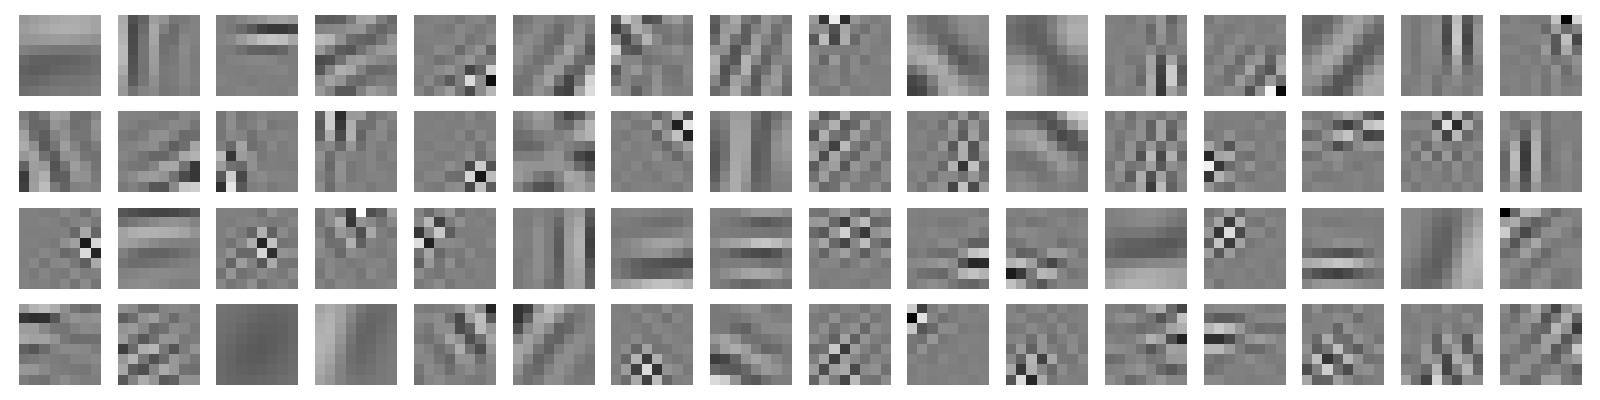
\includegraphics[width=\linewidth]{\toplevelprefix/chapters/chapter2/figs/msp_atoms_patches_new.png}
        \caption{}
    \end{subfigure}
    \begin{subfigure}{0.9\linewidth}
        \centering
        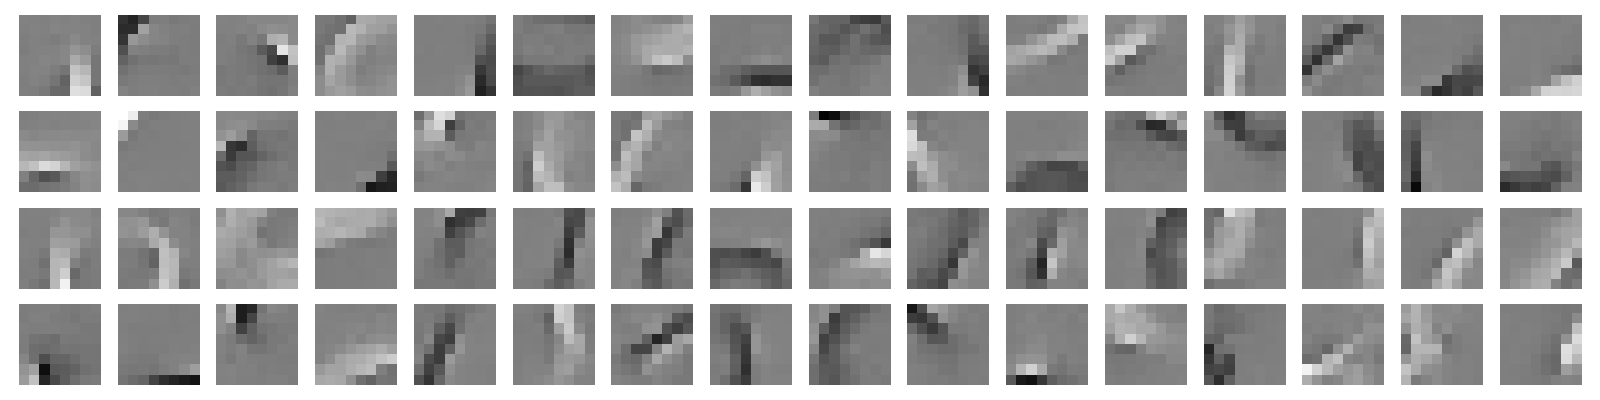
\includegraphics[width=\linewidth]{\toplevelprefix/chapters/chapter2/figs/palm_atoms_patches_new.png}
        \caption{}
    \end{subfigure}
    \caption{完备(正交)字典和过完备字典学习到的字典原子比较,训练用于重构从MNIST数字中提取的$8 \times 8$图像块。两个字典都在$10^4$个具有非平凡内容的随机图像块上训练了$6000$个周期,稀疏编码使用LASSO目标和$\lambda=0.1$计算(见 \eqref{eq:sparse_dl_lasso})。颜色图中黑色表示负值,白色表示正值。\textbf{上图:}使用MSP算法 \eqref{eq:msp_iteration} 学习的正交字典被限制为最多有$64$个原子;学习到的原子大致对应于一个“尖峰和平板”字典,在保留的测试数据上实现了相对较差的重构稀疏度水平(相对于$10^{-1}$的阈值,编码平均约为$17$-稀疏)。\textbf{下图:}相比之下,一个过完备字典(这里有$8^3$个原子;我们可视化了$64$个的随机子集)学习到了语义上有意义的字典原子,对应于带符号的有向边缘,这些原子可以拼接起来创建数字图像块,并实现更优的重构和稀疏度水平。编码平均约为$20$-稀疏,同时比正交字典的编码大$8$倍。为了计算字典,我们使用了一个基于近端交替线性化最小化的优化器,作用于一个适当正则化版本的\eqref{eqn:DL-overcomplete}。}
    \label{fig:ReconMNIST}
\end{figure}

事实上,过完备字典学习最初是作为一种生物学上合理的图像表示算法提出的,基于对视觉皮层早期阶段如何表示视觉刺激的经验证据 \cite{Olshausen1996-ap,Olshausen1997-yv}。

在本节的其余部分,我们将发展过完备字典学习的概念和计算基础。
与正交字典学习问题 \eqref{eqn:autoencoding-DL} 相类似,我们陈述了稀疏使用的过完备字典的压缩自编码问题。即,假设模型 \eqref{eq:model-DL-overcomplete} 对于数据 \(\vx\)、过完备字典 \(\vA\) 和稀疏度 \(d\) 成立,并且给定 \(\vx\) 的样本 \(\vX = [\vx_1, \dots, \vx_N]\),我们希望学习一个编码器 \(\cE : \R^D \to \R^m\) 将每个 \(\vx\) 映射到其\textit{稀疏编码} \(\vz\),以及一个解码器 \(\cD(\vz) = \vA \vz\) 从其稀疏编码重构每个 \(\vx\),使得 \(\cE(\vx)\) 和 \(\cD(\vz) = \vA\vz\) 构成 \(\vx\) 的一个有损自编码对。图示如下:
\begin{equation}
\x \xrightarrow{\hspace{4mm} \mathcal{E} \hspace{4mm}}  \z \xrightarrow{\hspace{2mm} \mathcal{D} = \vA \hspace{2mm}}   \hat{\x}.  
\label{eqn:autoencoding-DL-overcomplete}
\end{equation}    
我们将从编码器 $\cE$ 的构建开始。
我们将逐步进行:首先,\textit{给定真实的字典 $\vA$},我们将展示\textit{稀疏编码}问题如何给出一个优雅、可扩展且可证明正确的算法来恢复 $\vx$ 的稀疏编码 $\vz$。
虽然这个问题在最坏情况下是NP难的,但对于\textit{非相干}的字典 $\vA$(即列不太相关的字典),它可以被高效且可扩展地解决。
这个解决方案所包含的编码器架构将不再是对称的:我们将看到它具有一个原始深度网络的形式,该网络依赖于字典 $\vA$。
然后我们将继续学习解码器 $\cD$ 的任务,或者等价地,学习过完备字典 $\vA$。
我们将推导一个过完备字典学习的算法,该算法允许我们
同时学习码本 $\vA$ 和稀疏编码 $\vz$,利用稀疏编码的思想。
最后,我们将讨论一个关于可学习稀疏编码的更现代的视角,它将我们引向一个完全不对称的编码器-解码器结构,作为 \eqref{eqn:autoencoding-DL-overcomplete} 的替代方案。
在这里,解码器将对应于稀疏字典学习问题的增量解,并首次产生一对用于稀疏字典学习的类似深度网络的编码器解码器。
这种结构将预示着专著其余部分将要出现的许多发展。



%之前,我们将数据(在\(\R^{D}\)中)建模为来自一个子空间(第\ref{sec:lowrank}节)或最多\(D\)个子空间的混合(第\ref{sec:ica}节)。然而,这尚未涵盖数据具有线性结构的所有情况。考虑以下相关案例。假设我们有一个数据集\(\{\vx_{i}\}_{i = 1}^{N}\),其中数据共享某些特征;例如,假设它们都是卧室的自然图像。那么,几乎所有数据中都存在一组共同的、重复的\textit{主题}或\textit{模式}:墙壁涂料图案、床、梳妆台等。我们希望提取这些模式并理解它们如何组合形成数据。虽然这看起来像一个玩具例子,但它在图像处理中一直发生。著名的是,使用本章后续方法从自然图像数据中提取的模式与大脑在处理相同数据时发现的模式相似。\DP{引用bruno的论文,该论文应用DL从大脑数据中提取Gabor小波}
%
%更一般地,假设数据\(\vx_{i}\)都位于某个集合\(\cX \subseteq \R^{D}\)中(在上面的例子中,是卧室自然图像的集合)。为了通过数据分析从\(\vx_{i}\)中提取意义,我们构建了一组\(d\)个\textit{原子}\(\{\va_{i}\}_{i = 1}^{d} \subseteq \cX\),代表一些可解释的主题,使得没有\(\vx_{i}\)离一个原子或少数原子的简单(线性)组合太远,从而这些主题组合形成我们的数据。(这在形式化后被称为\textit{覆盖},数字\(d\)至少是\textit{覆盖数},通常远大于\(D\))。然后,我们希望恢复\(\vx_{i}\)到原子的编码。我们也可能希望在给定数据集的情况下提取一组最优的原子。这分别是稀疏编码和字典学习的目的。
%%\DP{稍后填写稀疏编码/字典学习的具体动机……我认为我给出的很多例子都相当复杂……}

\subsection{使用过完备字典进行稀疏编码} 

在本节中,我们将考虑一个容纳了许多主题或\textit{原子}的稀疏线性组合的数据模型。从机制上讲,这建议我们考虑以下数据模型。我们说数据\(\{\vx_{i}\}_{i = 1}^{N} \subseteq \R^{D}\)具有(近似)\(s\)-稀疏编码结构,当且仅当存在一个矩阵\(\vA = \mat{\va_{1}, \dots, \va_{d}} \in \R^{D \times d}\),向量\(\{\vz_{i}\}_{i = 1}^{N} \subseteq \R^{d}\)且对所有\(i\)都有\(\norm{\vz_{i}}_{0} \leq s\),以及小向量\(\{\veps_{i}\}_{i = 1}^{N} \subseteq \R^{D}\),使得
\begin{equation}\label{eq:vectorized_sparse_dl_dgp}
    \vx_{i} = \vA\vz_{i} + \veps_{i}, \qquad \forall i \in [N].
\end{equation}
注意稀疏编码结构和主成分结构之间的机制差异:1. 低维表示\(\vz_{i}\)被要求是\(s\)-稀疏的,2. \(\vA\)不被要求是正交的。

\(s\)-稀疏性条件来自于希望每个数据点都可以由少数\(s\)个原子(即\(\vA\)的列)的线性组合来表示。这本质上施加了数据分布的内在维度低于\(s\)的约束。

放宽正交性条件是因为,如我们上面的覆盖例子所示,\(d\)远大于\(D\),构建一个大小为\(D \times d\)的正交矩阵是不可能的。然而,字典\(\vA\),无论是给定的还是学习的,通常是\textit{非相干的},即乘积\(\va_{i}^{\top}\va_{j}\)通常很小,因此近似正交。\footnote{事实证明,在高维空间中,填充大量近似正交的向量是相当容易的,其数量远大于环境维度 \cite{Wright-Ma-2022}。}

注意,我们可以将\(\vx_{i}\)收集到\(\vX = \mat{\vx_{1}, \dots, \vx_{N}} \in \R^{D \times N}\)中,将\(\vz_{i}\)收集到\(\vZ = \mat{\vz_{1}, \dots, \vz_{N}} \in \R^{d  \times N}\)中,并将\(\veps_{i}\)收集到\(\vE = \mat{\veps_{1}, \dots, \veps_{N}} \in \R^{D \times N}\)中,以将\eqref{eq:vectorized_sparse_dl_dgp}重写为
\begin{equation}\label{eq:sparse_dl_dgp}
    \vX = \vA\vZ + \vE.
\end{equation}
我们考虑的第一个问题是:如果我们知道矩阵\(\vA\),并希望用\(\vA\)来表示我们的数据\(\vX\),该怎么办?这属于\textit{稀疏编码}的范畴。与完备字典学习类似,我们试图找到与我们的观测一致的最稀疏的信号,这自然地引出了以下优化问题:
\begin{equation}\label{eq:sparse_dl_lasso}
    \min_{\vZ \in \R^{d \times N}}\bc{\norm{\vX - \vA\vZ}_{2}^{2} + \lambda \norm{\vZ}_{1}},
\end{equation}
其中\(\ell^1\)范数\(\norm{\vZ}_{1}\)已知能促进解的稀疏性 \cite{Wright-Ma-2022}。
这个问题被称为LASSO问题。然而,与PCA或完备字典学习的情况不同,没有明确的幂迭代类型算法来恢复\(\vZ^{\ast}\)。一个自然的选择是考虑用梯度下降类型的算法来解决上述优化问题。设\(f(\vZ) = \norm{\vX - \vA\vZ}_{2}^{2} + \lambda \norm{\vZ}_{1}\)。从概念上讲,我们可以尝试用以下迭代来找到\(\vZ^{\ast}\):
\begin{equation}
    \vZ_{t+1} \leftarrow \vZ_t + \eta \nabla f(\vZ_t).
\end{equation}

然而,由于与\(\ell^1\)范数\(\norm{\vZ}_{1}\)相关的项是非光滑的,我们不能直接运行梯度下降。对于这类函数,我们需要用一个推广了梯度概念的东西,即次梯度\(\partial f(\vZ)\),来替换梯度\(\nabla f(\vZ)\):
\begin{equation}
    \vZ_{t+1} \leftarrow \vZ_t + \eta \partial f(\vZ_t).
\end{equation}
然而,众所周知,次梯度下降的收敛通常非常慢。因此,对于这类优化问题,通常采用所谓的\textit{近端梯度下降}类型的算法。读者可以参考\cite{Wright-Ma-2022}来详细了解这种方法。

将近端梯度应用于LASSO目标函数\eqref{eq:sparse_dl_lasso},会得到经典的\textit{迭代收缩-阈值算法}(ISTA),它实现以下迭代
\begin{eqnarray}
    \vZ_{1} &\sim& \dNorm(\vzero, \vI), \\
    \vZ_{t + 1} &=& S_{\eta\lambda}\rp{\vZ_{t} - 2\eta \vA^{\top}(\vA\vZ_{t} - \vX)}, \quad \forall t \geq 1,\label{eq:ista_update}
\end{eqnarray}
其中步长为\(\eta \geq 0\),软阈值算子\(S_{\alpha}\)在标量上定义为
\begin{equation}
    S_{\alpha}(x) \doteq \begin{cases}x - \alpha, & x \geq \alpha, \\ 0, & -\alpha < x < \alpha, \\ x + \alpha, & x \leq -\alpha\end{cases},
\end{equation}
并逐元素地应用于输入矩阵。作为一个应用于凸问题的近端梯度下降算法,收敛到全局最优是有保证的,并且收敛率可以被直接推导出来 \cite{Wright-Ma-2022}。

我们现在花点时间评论一下\eqref{eq:ista_update}中更新算子的函数形式,它具有以下形式
\begin{equation}
    \vZ_{t + 1} = \texttt{非线性}(\vZ_{t} + \texttt{线性}^{\top}(\texttt{线性}(\vZ_{t}) + \texttt{偏置})).
\end{equation}
这种函数形式与残差网络层的形式非常相似,即
\begin{equation}
    \vZ_{t + 1} = \vZ_{t} + \texttt{线性}_{1}^{\top}(\texttt{非线性}(\texttt{线性}_{2}(\vZ_{t}) + \texttt{偏置}_{1}) + \texttt{偏置}_{2},
\end{equation}
只是解耦了线性映射(即矩阵乘法),增加了一个偏置,并移动了非线性部分。因此,ISTA可以被看作是一个原始(循环单层)神经网络的前向传播。我们在第\ref{ch:representation}章中论证,这类操作对于深度表示学习至关重要。

% 低维线性独立结构的混合……Lasso和L1最小化。介绍稀疏编码的基本算法,如ISTA。

% \begin{itemize}
%     \item 将LASSO/L1的动机解释为:首先我们将ICA理解为多个子空间,其中我们每次只从少数子空间基向量中求和。现在,如果我们让子空间基向量的数量趋于\(\infty\)呢?或者非常大?就变成了稀疏表示问题。
%     \item 介绍LASSO和ISTA
%     \item 当我们有字典时,是LASSO和L1,当我们没有时,是过完备字典学习,讨论LISTA/KSVD等及其应用
% \end{itemize}


\subsection{过完备字典学习} 

回想一下,我们有数据模型
\begin{equation}
    \vX = \vA\vZ + \vE,
\end{equation}
其中\(\vZ\)是稀疏的,我们之前的目标是在给定数据\(\vX\)和字典原子\(\vA\)的情况下估计\(\vZ\)。现在我们转向更常见、更自然、也更困难的情况,即我们既不知道\(\vA\)也不知道\(\vZ\),并试图从一个大数据集中学习它们。具体来说,我们解决以下问题
\begin{equation}
    \min_{\tilde{\vA}, \tilde{\vZ}}\bc{\norm{\vX - \tilde{\vA}\tilde{\vZ}}_{F}^{2} + \lambda \norm{\tilde{\vZ}}_{1}}.
    \label{eqn:DL-overcomplete}
\end{equation}
\begin{remark}[$\ell^4$ 最大化与 $\ell^1$ 最小化]
注意,上述问题表述自然地源于稀疏编码的LASSO表述 \eqref{eq:sparse_dl_lasso}。我们通过最小化\(\ell^1\)范数来促进解的稀疏性。然而,如果我们只对恢复过完备字典\(\vA\)感兴趣,第 \ref{sec:complete-dictionary} 节中介绍的\(\ell^4\)最大化方案也推广到过完备情况,没有任何显著修改。感兴趣的读者可以参考 \cite{Qu2020Geometric} 的工作。
\end{remark}

上述问题 \eqref{eqn:DL-overcomplete},我们称之为\textit{过完备字典学习},是一个非凸问题,因为现在\(\vA\)和\(\vZ\)都是未知的。它不能用标准的凸优化工具包轻易解决。然而,因为它有趣、表述简单且在实践中很重要,已经有许多重要的工作致力于解决这个问题的不同算法和理论分析。在这里,为了本书的兴趣,我们提出一种解决这个问题的惯用方法,这种方法更接近深度学习的精神。

根据我们处理LASSO问题的经验,很容易看出,对于两个未知数\(\vA\)和\(\vZ\),如果我们固定一个并优化另一个,每个子问题实际上都是凸的并且容易解决。这自然地表明,我们可以尝试通过交替地对\(\vZ\)或\(\vA\)进行最小化来解决上述程序 \eqref{eqn:DL-overcomplete},例如使用梯度下降。这导致了以下迭代方案:
\begin{align}
    & \vZ^{1}
     \sim \dNorm(\vzero, \vI), \quad \vA_{1}
     \sim \dNorm(\vzero, \vI), \\ 
    &\vZ^{\ell + 1} = S_{\eta\lambda}\rp{\vZ^{\ell} - 2\eta\vA_{t}^{\top}(\vA_{t}\vZ^{\ell} - \vX)}, \qquad \forall \ell \in [L] \label{eqn:ISTA-update}\\ 
    &\vA_{t + 1} = \vA_{t} - 2\nu (\vA_{t}\vZ^{\ell + 1} - \vX)\vZ^{\ell + 1}, \qquad\;\; \forall t \in [T].\label{eqn:DL-update}
\end{align}
这里,与典型的交替最小化方案不同,我们使用两个独立的索引 $\{t\}$ 和 $\{\ell\}$ 来表示迭代。正如我们稍后将看到的,这使我们能够在深度学习的背景下分别解释这两个更新。尽管字典学习问题是一个非凸问题,但已经证明,上述交替最小化类型的算法确实会收敛到正确的解,至少是局部地,例如参见 \cite{alekh-2016}。

%\yima{Sam,请将此修复为解决过完备字典学习问题的普通算法。陈述关于理解这种方法正确性的结果……完成本小节。}

\subsection{学习型深度稀疏编码}
\label{sec:LISTA}
上述方法的主要观察是注意到\textit{当我们固定\(\vA\)时,$\vZ^\ell$的ISTA更新\eqref{eqn:ISTA-update}看起来像一个深度神经网络的前向传播,其权重由\(\vA\)(和\(\vA^{\top}\))给出}。但通常情况下,我们不知道真实的$\vA_o$,当前的估计$\vA_t$可能有误。因此,需要根据使用当前$\vA_t$和$\vZ^{\ell +1}$恢复$\vX$的残差,使用\eqref{eqn:DL-update}进一步更新它。


\paragraph{逐层学习的稀疏编码。}
因此,如果我们将每个ISTA更新\eqref{eqn:ISTA-update}看作一个层,并允许相关的字典(现在表示为$\vA_t^\ell$)随时间更新,这就导致了一个“逐层可学习”的稀疏编码方案:
\begin{align}
    & \vZ^{\ell + 1} = S_{\eta\lambda}\rp{\vZ^{\ell} - 2\eta\vA_{t}^{\ell\top}(\vA_{t}^\ell\vZ^{\ell} - \vX)}, \quad \forall \ell \in [L] \\ 
    & \vA_{t + 1}^\ell = \vA_{t}^\ell - 2\nu (\vA_{t}^\ell\vZ^{\ell + 1} - \vX)\vZ^{\ell + 1}, \qquad \forall t \in [T].
\end{align}
\(L\)个内部步骤中的每一个都可以被认为是一个单层前向传播,而\(T\)个外部步骤中的每一个都可以被认为是一个原始深度神经网络的单层反向传播。特别是,这个算法是前向优化和反向学习之间出现明确分界的最简单情况。这种分界在当前的神经网络中仍然可以观察到。

\paragraph{学习型ISTA。} 上述交替最小化的深度网络解释更多是概念性的而非实用性的,因为这个过程可能相当低效,需要很多层或迭代才能收敛。但这主要是因为我们试图从\(\vX\)中同时推断\(\vZ\)和\(\vA\)。如果只用它们从一组给定的输入输出样本\((\vX, \vZ)\)中学习\(\vA^\ell\),问题可以被显著简化,上述迭代也可以变得更高效:
\begin{align}
    & \vZ^{\ell + 1} = S_{\eta\lambda}\rp{\vZ^{\ell} - 2\eta(\vA^{\ell})^{\top}(\vA^\ell\vZ^{\ell} - \vX)}, \quad \forall \ell \in [L].
\end{align}
如果我们将每次迭代的算子表示为$\vZ^{\ell + 1} = f(\vA^\ell, \vZ^\ell)$,上述迭代可以用一个图表来说明:
\begin{equation*}
\vX, \vZ^1 \xrightarrow{\hspace{1mm} f(\vA^1,\,\cdot\,) \hspace{1mm}}  \vZ^2 \xrightarrow{\hspace{1mm} f(\vA^2,\,\cdot\,) \hspace{1mm}}  \vZ^3  \xrightarrow{\hspace{1mm} f(\vA^3,\,\cdot\,) \hspace{1mm}} \cdots \vZ^{L}  \xrightarrow{\hspace{1mm} f(\vA^{L},\,\cdot\,) \hspace{1mm}} \vZ^{L + 1} \approx \vZ.  
\label{eqn:deep-sparse-encoding}
\end{equation*}

因此,给定这个序列结构,为了学习每一层的算子\(\vA^\ell\),通过最小化最终编码$\vZ^L$与真实值$\vZ$之间的误差,例如通过反向传播(BP)\footnote{关于BP的简要描述,请参见附录\ref{app:optimization}。}来学习它是完全自然的:
\begin{equation}
    \min_{\{\vA^\ell\}} \big\|\vZ^L(\vA^1, \ldots, \vA^{L}) - \vZ\big\|_2^2.
\end{equation}
这是学习型ISTA(LISTA)算法\cite{gregor2010learning}的基础,它可以被看作是一个深度神经网络的学习算法,该网络试图模拟从$\vX$到$\vZ$的稀疏编码过程。特别是,它可以被看作是一个\textit{简单的表示学习算法}。
%\yima{可能需要用伪代码形式写出LISTA算法。}


LISTA的经验成功引出了一个问题:如果我们使用逐层不同的字典\(\vA^\ell\)来编码更复杂的数据,并通过反向传播学习权重,会怎么样?这\textit{正是}深度(线性)神经网络背后的思想。我们将在后续章节中更多地讨论这一点。

% 低维线性独立结构的混合,不知道编码……L4最大化。我们在完备情况下的工作:\href{https://arxiv.org/abs/1906.02435}{基于L4的字典学习}





\section{总结与注释}


\sdb{添加一些简短的总结和一个总结幂方法的表格。也许这个部分应该放在本章的末尾,与自编码总结表一起?}

\textit{独立成分分析}(ICA),由\cite{Ans-1985}提出,并由Aapo Hyv\"{a}rinen在1990年代和2000年代初开创。

统一的计算机制:通过基于一阶预言机(梯度)的\textit{幂迭代}来追求低维线性和独立模型。

提及早期使用自联想或自编码神经网络学习PCA的历史,以及Qing小组最近关于通过扩散学习PCA的工作。

提及John Wright和Qing Qu等人在过完备字典学习方面的工作。

提及早期对多个子空间的推广(例如GPCA)及其局限性,以及与后面关于率失真(Rate Reduction)的章节的联系。


\section{练习与扩展}


\begin{exercise}\label{exercise:principal-components-derivation}
    证明,对于任何对称矩阵\(\vA\),问题\(\max_{\vU \in \O(D, d)}\tr\left(\vU^{\top}\vA\vU\right)\)的解是矩阵\(\vU^{\ast}\),其列是\(\vA\)的前\(d\)个单位特征向量。
\end{exercise}

\begin{exercise}\label{exercise:gaussian-rot-invar}
    设$\vz \sim \cN(\Zero, \sigma^2 \vI)$为一个高斯随机变量,其分量独立,每个分量的方差为$\sigma^2$。
    证明对于任何正交矩阵$\vQ$(即$\vQ^\top \vQ = \vI$),随机变量$\vQ \vz$与$\vz$的分布相同。
    \textit{(提示:回想高斯概率密度函数的公式,以及随机变量线性函数的密度公式。)}
\end{exercise}

\begin{exercise}\label{exercise:symmetry-identifiability}
    上面讨论的统计可识别性概念可以与模型类的\textit{对称性}联系起来,从而允许在没有任何统计假设的情况下,以纯粹确定性的方式理解估计。

    考虑模型$\vX = \vU \vZ$,其中$\vX, \vU, \vZ$是尺寸兼容的矩阵。
    \begin{enumerate}
        \item 证明如果$\vA$是任何尺寸兼容的方阵可逆矩阵,那么对
        $(\vU \vA, \vA^{-1} \vZ)$在模型下也等于$\vX$。我们称之为\textit{$\GL(d)$对称性}。
        \item 假设$\vZ$的每一列都是来自一个共同统计模型$\vz$的独立同分布观测,此外$\vz$的均值为零,分量$z_i$独立且方差为正。
        证明对于任何方阵可逆矩阵$\vA$,如果$\vA \vz$的分量不相关,那么$\vA$可以写成$\vD_1 \vQ \vD_2$的形式,其中$\vQ$是一个正交矩阵,$\vD_1, \vD_2$是对角矩阵。
        \textit{这将ICA中的“独立性”假设与“对称性破缺”效应联系起来,后者只允许尺度和旋转对称性。}
    \end{enumerate}

\end{exercise}

\begin{exercise}\label{exercise:whitening}
    考虑模型$\vx = \vU \vz$,其中$\vU \in \R^{D \times d}$($D \geq d$)是固定的且秩为$d$,$\vz$是一个零均值随机变量。设$\vx_1, \dots \vx_N$表示来自该模型的独立同分布观测。
    \begin{enumerate}
        \item 证明矩阵$\vX = [\vx_1, \dots, \vx_N]$的秩不大于$d$,因此存在一个标准正交矩阵$\vV \in \R^{D \times d}$使得$\vX = \vV \vY$,其中$\vY \in \R^{d \times N}$。(\textit{提示:使用PCA。})
        \item 证明\textit{白化矩阵}$(\vY \vY^\top)^{-1/2}\vY$在$\Cov(\vz)$非奇异时在期望意义下存在,并且其经验协方差为单位矩阵。\footnote{特别地,可以从数学上证明,只要$\vz$满足适当的集中不等式且$N$足够大,这就足以保证白化矩阵以高概率存在。}
        \item 使用$\vU$的奇异值分解,证明可以选择矩阵$\vV$,使得白化矩阵满足$(\vY \vY^\top)^{-1/2} \vY = \vW [\vz_1, \dots, \vz_N]$,其中$\vW$是一个标准正交矩阵。
    \end{enumerate}
\end{exercise}

\begin{exercise}\label{exercise:kurtosis-linearity-properties}
    设$X$和$Y$是零均值的独立随机变量。
    \begin{enumerate}
        \item 证明$\kurt(X + Y) = \kurt(X) + \kurt(Y)$。
        \item 对于任何$\alpha \in \R$,证明$\kurt(\alpha X) = \alpha^4 \kurt(X)$。
    \end{enumerate}
\end{exercise}

\begin{exercise}\label{exercise:sphere-calculus}
    设$f : \R^d \to \R$是一个给定的二次连续可微目标函数。考虑球约束优化问题
    \begin{equation}\label{eq:exercise-sphere-constrained-max}
        \max_{\norm{\vu}_2^2 = 1}\, f(\vu). 
    \end{equation}
    在本练习中,我们将推导我们在FastICA推导中给出的、通过梯度上升算法在球面上最大化峰度的表达式。
    这些表达式是流形上微积分和优化丰富理论的特例,球面是其中的一个例子。对该领域的深入技术研究超出了我们的目的范围,因此我们只为感兴趣的读者提及两个关键参考文献:Absil、Mahony和Sepulchre的开创性教科书
    \cite{Absil2009-nc},以及Boumal最近的一本入门性论著 \cite{Boumal2023-rj}。
    \begin{enumerate}
        \item 对于任何作为$\R^d$的可微子流形的约束集$\cM$,在点$\vu \in \cM$处的
        \textit{切空间},非正式地讲,是流形$\cM$在点$\vu$处的最佳局部线性近似。
        在一个重要的特例中,当$\cM$在$\vu$处局部地定义为函数$F : \R^d \to \R$的水平集时,
        即
        \begin{equation*}
            U \cap \cM = F^{-1}(\set{0})
        \end{equation*}
        对于某个开集$U \subset \cM$且$\vu \in U$,
        $\cM$在$\vu$处的切空间可以通过
        微分计算:
        \begin{equation*}
            T_{\vu} \cM = \Ker(DF_{\vu}).
        \end{equation*}
        很容易看出,球面具有定义方程$F(\vu) = \norm{\vu}_2^2 - 1$。
        使用这些事实,证明在$\vu$处的球面切空间由下式给出
        \begin{equation*}
            T_{\vu} \bS^{d-1} = \set{\vv \in \R^d \given \ip{\vv}{\vu} = 0},
        \end{equation*}
        并且到该子空间的正交投影是$\vP_{\vu}^\perp = \vI - \vu\vu^\top$。
        \item 向量场
        \begin{equation}\label{eq:exercise-riemann-grad-sphere}
        \mathrm{grad}\, f(\vu) = \vP_{\vu}^\perp \nabla f
        \end{equation}
        被称为限制在球面上的函数$f$的\textit{黎曼梯度}。
        优化问题\eqref{eq:exercise-sphere-constrained-max}的\textit{一阶最优性条件}可以用黎曼梯度表示:
        \begin{equation*}
            \mathrm{grad}\, f(\vu) = \mathbf{0}.
        \end{equation*}
        从几何上看,这表示$f$在$\vu$处的欧几里得梯度必须与$\vu$处的球面切空间正交。
        现在假设$\vv \in \R^d$非零。证明
        \begin{equation*}
            \mathrm{proj}_{\bS^{d-1}}(\vv) :=
            \min_{\norm{\vu}_2^2 = 1}\, \norm{\vu - \vv}_2 
            =
            \frac{\vv}{\norm{\vv}_2},
        \end{equation*}
        使用一阶最优性条件。
        \item 在$\R^d$上的优化中,人们使用\textit{海森矩阵}$\nabla^2 f(\vu)$来检查二阶最优性条件(以确定临界点是最大值、最小值还是鞍点)。
        通过对球面的黎曼梯度$\mathrm{grad}\, f(\vu)$关于$\vu$求导(如本练习第一部分所示),证明用于确定球面约束优化的二阶最优性条件的相应对象是\textit{黎曼海森矩阵},定义为
        \begin{equation}\label{eq:exercise-riemann-hess-sphere}
            \mathrm{Hess}\, f(\vu) = \vP_{\vu}^\perp \left( 
            \nabla^2 f(\vu) - \ip{\nabla f(\vu)}{\vu} \vI
            \right) \vP_{\vu}^\perp.
        \end{equation}
    \end{enumerate}
\end{exercise}

\begin{exercise}\label{exercise:kurtosis-sphere-landscape}
    在本练习中,我们勾勒一个在文献中被称为\textit{景观分析}的论证,针对球约束总体峰度最大化问题\eqref{eq:kurtosis-maximization-sphere-population-simple}。我们将证明,当至少有一个独立分量具有正峰度时,其
    全局最大化点确实导致恢复字典$\vU$的一列。
    为简单起见,我们将假设对于每个$i = 1, \dots, d$,$\kurt(z_i) \neq 0$。
    \begin{enumerate}
        %\item 使用运行假设$\Var(z_i) = 1$,证明$\kurt(z_i) = \bE[z_i^4] - 3$。
        \item 使用练习\ref{exercise:sphere-calculus}第一部分的结果,
        证明\eqref{eq:kurtosis-maximization-sphere-population-simple}的一阶最优性条件是
        \begin{equation}\label{eq:kurtosis-sphere-landscape-stationarity}
            \left(\sum_{i=1}^d \kurt(z_i) w_i^4 \right) 
            \vw = \kurt(\vz) \hada \vw^{\hada 3}, 
        \end{equation}
        其中峰度是逐元素计算的,$\hada$表示向量的逐元素乘法,$\vw^{\hada 3}$表示其参数的逐元素立方。
        \item 证明满足\eqref{eq:kurtosis-sphere-landscape-stationarity}且单位范数的向量$\vw$
        都具有以下形式。
        设$S^+ = \set{i \in [d] \given \kurt(z_i) > 0}$,
        $S^- = \set{i \in [d] \given \kurt(z_i) < 0}$。
        设$S$是$S^+$或$S^-$的一个子集。
        那么
        \begin{equation}\label{eq:kurtosis-sphere-landscape-cps}
            \vw_S = \sum_{i \in S} \pm \sqrt{\frac{1}{\kurt(z_i) \sum_{j \in S} \frac{1}{\kurt(z_j)}}} \ve_i
        \end{equation}
        满足\eqref{eq:kurtosis-sphere-landscape-stationarity},
        其中$\ve_i$是在第$i$个位置为$1$、其他位置为$0$的向量,$\pm$符号表示选择正号或负号。
        \item 假设至少有一个$i$使得$\kurt(z_i) > 0$。使用练习\ref{exercise:sphere-calculus}第二部分的结果,证明\eqref{eq:kurtosis-maximization-sphere-population-simple}目标函数的唯一局部最大值是带符号的单稀疏向量$\pm \ve_i$,其中$i \in S^+$。结论是\eqref{eq:kurtosis-maximization-sphere-population-simple}的全局最大化点是对应于具有最大峰度的分量的带符号单稀疏向量。%
        %设$S_{\max} = \argmax_{i \in [d]}\, \kurt(z_i)$为具有最大峰度的独立分量的索引集。那么对于每个$i \in S_{\max}$,$\pm \ve_i$是\eqref{eq:kurtosis-maximization-sphere-population-simple}的一个局部最大化点。
        (\textit{提示:计算每个临界点处黎曼海森矩阵\eqref{eq:exercise-riemann-hess-sphere}的正负特征值的数量。})
        %\item 证明在任何临界点$\vw_S$处,\eqref{eq:kurtosis-maximization-sphere-population-simple}的目标函数值由下式给出
        %\begin{equation*}
        %    \frac{1}{\sum_{i \in S} \frac{1}{\kurt(z_i)}}.
        %\end{equation*}
        %\item 结论是
        \item 现在假设对于每个$j =1, \dots, d$,$\kurt(z_j) < 0$。这对应于峰度最大化问题的一个“过度收缩”实例。再次使用练习\ref{exercise:sphere-calculus}第二部分的结果,证明\eqref{eq:kurtosis-maximization-sphere-population-simple}目标函数的唯一局部最大值是带符号的稠密向量$\sum_{i=1}^d \pm \ve_i$。
        这表明优化公式\eqref{eq:kurtosis-maximization-sphere-population-simple}不能被天真地应用。
    \end{enumerate}
\end{exercise}

\begin{exercise}\label{exercise:fast-ica-convergence}
    \sdb{fastica的收敛性,基于\cite{hyvarinen-1997},第3.2节} 
\end{exercise}

%\begin{exercise}\label{exercise:orthogonal-dl-simplifying}
%    \sdb{简化正交DL LASSO损失……$\ell^2$的旋转不变性,然后是可分性,然后是Huber计算}
%\end{exercise}

\begin{exercise}\label{exercise:orthogonal-group-calculus}
    本练习遵循练习\ref{exercise:sphere-calculus}中介绍的结构和形式,但将其应用于正交群$\O(d) = \set{\vU \in \R^{d \times d} \given \vU^\top \vU = \vI}$。
    请参考练习\ref{exercise:sphere-calculus}的描述以获取必要的概念背景;只要记住矩阵上的相关内积是$\ip{\vX}{\vY} = \tr(\vX^\top \vY)$,该形式同样适用于环境空间是$d \times d$矩阵集的情况。
    关于正交群上优化的一个优秀的通用参考文献是Edelman、Arias和Smith的\cite{Edelman1998-lg}。
    
    设$f : \R^{d\times d} \to \R$是一个给定的二次连续可微目标函数。考虑正交约束优化问题
    \begin{equation}\label{eq:exercise-orthogonal-group-constrained-max}
        \max_{\vQ^\top \vQ = \vI}\, f(\vQ). 
    \end{equation}
    \begin{enumerate}
        \item 很容易看出,正交群具有定义方程$F(\vQ) = \vQ^\top \vQ = \vI$。
        使用这个事实,证明在$\vQ$处的正交群切空间由下式给出
        \begin{equation*}
            T_{\vQ} \O(d) = \set{\vQ \vOmega \in \R^{d\times d} \given \vOmega^\top = - \vOmega},
        \end{equation*}
        并且到该子空间的正交投影是
        \begin{equation*}
        \cP_{T_{\vQ}\O(d)}(\vDelta) =  \vQ \Skew(\vQ^\top \vDelta),
        \end{equation*}
        其中$\Skew(\vDelta) = \tfrac{1}{2} ( \vDelta - \vDelta^\top)$是到斜对称矩阵集上的正交投影。
        向量场
        \begin{equation}\label{eq:exercise-riemann-grad-orthogonal-group}
        \mathrm{grad}\, f(\vQ) = \cP_{T_{\vQ} \O(d)} \left( \nabla f(\vQ) \right)
        \end{equation}
        被称为限制在正交群上的函数$f$的\textit{黎曼梯度}。
        优化问题\eqref{eq:exercise-orthogonal-group-constrained-max}的\textit{一阶最优性条件}可以用黎曼梯度表示:
        \begin{equation*}
            \mathrm{grad}\, f(\vQ) = \mathbf{0}.
        \end{equation*}
        \item 通过对正交群的黎曼梯度$\mathrm{grad}\, f(\vQ)$关于$\vQ$求导(如本练习第一部分所示),证明\textit{黎曼海森矩阵}由下式给出
        \begin{equation}\label{eq:exercise-riemann-hess-orthogonal-group}
            \mathrm{Hess}\, f(\vQ) = \cP_{T_{\vQ}\O(d)} \left( 
            \nabla^2 f(\vQ) - \Symm(\vQ\adj \nabla f(\vQ)) \kron \vI
            \right) \cP_{T_{\vQ}\O(d)},
        \end{equation}
        其中$\Symm(\vDelta) = \tfrac{1}{2}(\vDelta + \vDelta^\top)$表示到对称矩阵集上的正交投影,$\kron$表示矩阵的克罗内克积。
        注意将前面表达式中出现的算子解释为\textit{作用于${d \times d}$矩阵的线性变换},\textbf{而不是}作为$d \times d$矩阵本身。
        优化问题\eqref{eq:exercise-orthogonal-group-constrained-max}的\textit{二阶最优性条件}可以用黎曼海森矩阵表示:
        \begin{equation*}
            \mathrm{Hess}\, f(\vQ) \preceq \mathbf{0}.
        \end{equation*}
        对于最小化问题,符号相反。

        (\textit{提示:关键是操纵你的计算以获得\eqref{eq:exercise-riemann-hess-orthogonal-group}的形式,使其尽可能紧凑。为此,利用克罗内克积的以下同构性:如果$\vA, \vX, \vB$是尺寸兼容的矩阵,那么有
        \begin{equation*}
            (\vB\adj \kron \vA) \Vec(\vX) = \Vec(\vA \vX \vB),
        \end{equation*}
        其中$\Vec(\vX)$表示将矩阵参数的列“从左到右”堆叠成一个向量。我们在\eqref{eq:exercise-riemann-hess-orthogonal-group}中使用这个同构性,以便以一种规范的方式将两个矩阵的克罗内克积定义为作用于矩阵的算子。})
        
        \item 现在假设$\vX \in \R^{d\times d}$是满秩的。在本练习的这一部分和下一部分,我们考虑$\vX$到正交群上的投影:
        \begin{equation}\label{eq:projection-onto-ogrp-defn}
            \mathrm{proj}_{\O(d)}(\vX) :=
            \min_{\vQ \in \O(d)
            }\, \norm{\vQ - \vX}_F^2.
        \end{equation}
        我们将证明这个问题的解由下式给出
        \begin{equation*}
            \mathrm{proj}_{\O(d)}(\vX)
            =
            \vU \vV^\top,
        \end{equation*}
        其中$\vX = \vU \vS \vV^\top$是$\vX$的奇异值分解。

        \begin{enumerate}
            \item 使用一阶和二阶最优性条件,证明\eqref{eq:projection-onto-ogrp-defn}的每个局部最小化点$\vQ$都满足
            \begin{align*}
                \left( \vQ^\top \vX \right)^\top &= \vQ^\top \vX, \\
                \vQ^\top \vX &\succeq \mathbf{0}.
            \end{align*}
            (\textit{提示:在两个参数中的一个固定时,利用克罗内克积的线性性。})
            \item 使用这些条件,论证在\eqref{eq:projection-onto-ogrp-defn}的每个局部最小化点$\vQ$处,有$\vQ^\top \vX = (\vX^\top \vX)^{1/2}$。
            %实现的损失值为$\norm{(\vX\adj \vX)^{1/2} - \vI}_F^2$。
            (\textit{提示:使用%$\ell^2$范数的酉不变性和
            线性代数中的一个事实,即如果$\vS \succeq \mathbf{0}$是一个对称半正定矩阵,那么$(\vS^\top\vS)^{1/2} = \vS$。})
            \item 使用奇异值分解$\vX = \vU \vS \vV^\top$,得出结论
            \begin{equation*}
                \vU \vV^\top
                =
                \mathrm{proj}_{\O(d)}(\vX).
            \end{equation*}
        \end{enumerate}
    \end{enumerate}
\end{exercise}

% \begin{exercise}\label{exercise:l4-global-maximizers-ogrp}
% %\sdb{推导$\ell^4$目标全局最大化点的练习。遵循Simon的论文/初等论证。}
% \end{exercise}

%\begin{exercise}\label{exercise:l4-maximizers-ogrp}
%    正如我们所见,在正交群上进行$\ell^4$最大化的一阶最优性条件(方程\eqref{eq:l4-ogrp-fxp-step1})可以写成如下形式:一个点$\vQ$是目标函数的临界点,当且仅当
%    \begin{equation}\label{eq:l4-ogrp-fxp-exercise-1}
%        \vX \left( \vX \adj \vQ \right)^{\hada 3} = \vQ \underbrace{\left. \left(
%        \vQ\adj \vX \left( \vX \adj \vQ \right)^{\hada 3} 
%        + 
%        \left( \vQ\adj \vX \right)^{\hada 3} \vX\adj \vQ
%        \right) \right/ 2}_{\vS}.
%    \end{equation}
%    在本练习中,我们将证明由这个条件定义的对称矩阵$\vS$在目标函数的任何最大化点处都是半正定的。
%    下面,为简洁起见,我们写成$f(\vQ) = \norm{\vX\adj \vQ}_4^4$。
%    \begin{enumerate}
%        \item 使用练习\ref{exercise:orthogonal-group-calculus}中推导的在正交群上的黎曼海森矩阵表达式\eqref{eq:exercise-riemann-hess-orthogonal-group},论证一个点$\vQ$是$\ell^4$最大化问题局部最大化点的必要条件是$\vQ$满足\eqref{eq:l4-ogrp-fxp-exercise-1}并且
%        \begin{equation*}
%            \cP_{T_{\vQ}\O(d)}
%            \left(
%             \vQ\adj \nabla f(\vQ) \kron \vI
%             \right)
%            \cP_{T_{\vQ}\O(d)}
%            \succeq \mathbf{0}.
%        \end{equation*}
%        \item 使用克罗内克积的定义,论证前一个条件等价于以下条件:对于任何斜对称矩阵$\vOmega$(即$\vOmega\adj = -\vOmega$),有
%        \begin{equation*}
%            \ip*{\vOmega}{
%             \vOmega \vQ\adj \nabla f(\vQ)
%             }
%            \geq 0.
%        \end{equation*}
%        (\textit{提示:回想练习\ref{exercise:orthogonal-group-calculus}中正交群的切空间的定义。})
%        \item 根据线性代数中的谱定理,任何斜对称矩阵$\vOmega$(作为一个正规矩阵)都有一个特征值分解$\vOmega = \vV \vLambda \vV\adj$,其中$\vV \in \C^{d \times d}$是一个酉矩阵,$\vLambda \in \C^{d\times d}$是一个对角特征值矩阵。
%        证明实值斜对称矩阵$\vOmega \in \R^{d \times d}$的以下表征:$\vOmega\adj = -\vOmega$当且仅当$\vOmega = \vV \vLambda \vV\adj$,其中酉矩阵$\vV$和对角矩阵$\vLambda$具有以下对称性:
%        \begin{itemize}
%            \item 所有特征值$\lambda_i$都是纯虚数,即$\mathfrak{R}(\lambda_i) = 0$。
%            \item 当$d$是偶数时,特征值$\lambda_i$可以被划分为对,具有以下性质。如果$(i, j)$是划分中的一对索引,则有$\lambda_i = -\lambda_j$。当$d$是奇数时,可以形成相同的划分,但有一个额外的奇数个索引$i$使得$\lambda_i = 0$。
%            \item 与这个划分中每对非零特征值相关联的相应特征向量$\vv_i$和$\vv_j$满足$\vv_i = \ol{\vv_j}$,其中$\ol{z}$表示复数$z$的共轭(逐元素应用于复向量)。
%            与零特征值相关联的特征向量是任意的,只要矩阵$\vV$是酉的。
%        \end{itemize}
%        \item 使用前面斜对称矩阵的表征和$\ell^4$最大化问题局部最大值的先前条件,
%        得出结论,在任何局部最大值$\vQ$处,必须有
%        \begin{equation*}
%            \vQ\adj \nabla f(\vQ) \succeq \mathbf{0}. 
%        \end{equation*}
%        (\textit{提示:如果$\vOmega$是斜对称的,那么根据前一部分的表征,半正定矩阵$\vOmega\adj \vOmega$的特征值可以被划分为值相等的对。如果$\vv$是与这个(非零)对相关联的特征向量,证明$\mathfrak{R}(\vv)$和$\mathfrak{I}(\vv)$(适当归一化后)可以被选为$\vOmega\adj \vOmega$的相应特征向量。给定一个推定的局部最大值$\vQ$使得$\vQ\adj \nabla f(\vQ) \not \succeq \mathbf{0}$,使用这个构造来推导一个矛盾。})
%        \sdb{这个论证还有问题……似乎最多只能证明1个负特征值(斜对称对)……对于这个声明还需要更多($\det(\nabla f(\vQ)) = \det(\vQ)$……)}
%    \end{enumerate}
%\end{exercise}

\end{document}